% arara: pdflatex
% arara: pdflatex
% arara: pdflatex

% options:
% thesis=B bachelor's thesis
% thesis=M master's thesis
% czech thesis in Czech language
% slovak thesis in Slovak language
% english thesis in English language
% hidelinks remove colour boxes around hyperlinks

\documentclass[thesis=B,czech]{FITthesis}[2012/06/26]

%\usepackage[utf8]{inputenc} % LaTeX source encoded as UTF-8

\usepackage{graphicx} %graphics files inclusion
% \usepackage{amsmath} %advanced maths
% \usepackage{amssymb} %additional math symbols
\usepackage{xevlna}
\usepackage{float}

\usepackage{multirow}

\usepackage{dirtree} %directory tree visualisation

\usepackage{listings}

\renewcommand{\lstlistingname}{Ukázka kódu}
\newcommand{\quoting}[1]{\textit{\uv{#1}}}
\usepackage{rotating}
\usepackage{color}
\usepackage{hyperref}
\usepackage{subcaption}
\usepackage{incgraph,tikz}

\usepackage[font=small,labelfont=bf]{caption}

\definecolor{dkgreen}{rgb}{0,0.6,0}
\definecolor{gray}{rgb}{0.5,0.5,0.5}
\definecolor{mauve}{rgb}{0.58,0,0.82}

\lstset{frame=tb,
  language=C,
  aboveskip=3mm,
  belowskip=3mm,
  showstringspaces=false,
  columns=flexible,
  basicstyle={\small\ttfamily},
  numbers=none,
  numberstyle=\tiny\color{gray},
  keywordstyle=\color{blue},
  commentstyle=\color{dkgreen},
  stringstyle=\color{mauve},
  breaklines=true,
  breakatwhitespace=true,
  tabsize=3
}

% % list of acronyms
% \usepackage[acronym,nonumberlist,toc,numberedsection=autolabel]{glossaries}
% \iflanguage{czech}{\renewcommand*{\acronymname}{Seznam pou{\v z}it{\' y}ch zkratek}}{}
% \makeglossaries

\newcommand{\tg}{\mathop{\mathrm{tg}}} %cesky tangens
\newcommand{\cotg}{\mathop{\mathrm{cotg}}} %cesky cotangens

% % % % % % % % % % % % % % % % % % % % % % % % % % % % % % 
% ODTUD DAL VSE ZMENTE
% % % % % % % % % % % % % % % % % % % % % % % % % % % % % % 

\department{Katedra číslicového návrhu}
\title{Robotická ruka}
\authorGN{Ilia} %(křestní) jméno (jména) autora
\authorFN{Popov} %příjmení autora
\authorWithDegrees{} %jméno autora včetně současných akademických titulů
\author{Ilia Popov} %jméno autora bez akademických titulů
\supervisor{Ing. Miroslav Skrbek, Ph.D.}
\abstractCS{
Cílem této práce bylo prozkoumat model robotické ruky od společnosti YouBionic a následně navrhnout a implementovat programové vybavení pro ovládání.


V práci je podrobně popsán původní produkt, který byl pak modernizován jak hardwarově tak i softwarově. Pro ovládání modelu pohybem paže uživatele byla vytvořena rukavice se senzory ohybu. 


Také bylo v práci implementováno programové řešení pro řídící jednotku robotické ruky a vytvořena PC aplikace v jazyce C pro ovládání a demonstraci možností modelu.
}
\abstractEN{
The goal of this thesis was to study a model of a robotic hand from the company YouBionic and then to design and implement software to control this product.

This thesis in detail describes the original product, which was then upgraded in terms of both hardware and software. A glove with flex sensors was created to control the model by moving the user's arm.


Software solution involved creating script for the control unit of the robotic hand and PC application in C language to control and demonstrate its capabilities.
}
\placeForDeclarationOfAuthenticity{V~Praze}
\declarationOfAuthenticityOption{5} %volba Prohlášení (číslo 1-6)
\keywordsCS{Robotická ruka, YouBionic Hand, Arduino, servomotor, Ohybový senzor, programové vybavení}
\keywordsEN{Robotic hand, YouBionic Hand, Arduino, servo, humanoid, Flex sensor, software}
\acknowledgements{


Chtěl bych poděkovat panu Ing. Miroslavu Skrbkovi, Ph.D. za vedení, trpělivost a praktickou pomoc v rámci této bakalářské práce.
Dále děkuji Bc. Petrovi Guľovi za technickou pomoc v laboratoři, své kamarádce Janě za rady v české gramatice a své rodině za podporu a pomoc při studiu.}
% \website{http://site.example/thesis} %volitelná URL práce, objeví se v tiráži - úplně odstraňte, nemáte-li URL práce


\renewcommand{\labelitemi}{---}

\begin{document}

% \newacronym{CVUT}{{\v C}VUT}{{\v C}esk{\' e} vysok{\' e} u{\v c}en{\' i} technick{\' e} v Praze}
% \newacronym{FIT}{FIT}{Fakulta informa{\v c}n{\' i}ch technologi{\' i}}

\begin{introduction}


Robotika je dnes jednou z nejrychleji rostoucích oblastí. Součástí této oblasti je vývoj robotických ruk, které se v poslední době aktivně rozvíjejí. V podstatě jakékoli zařízení používané k pohybu objektů lze označit za robotickou ruku. Výhodou podobných zařízení je vysoká přesnost, proto se robotické ruce aktivně používají v průmyslu.


Další oblast je medicína. Robotické ruce se používá v chirurgii a jako protézy lidských končetin. Ve vývoji robotických ruk došlo k obrovskému pokroku díky rozvoji 3D tisku, který mnohokrát zlevnil výrobu podobných projektů.


Mechanický model je pouze jednou částí těchto projektů, druhou částí je software. Model musíme naprogramovat, abychom jej mohli podle potřeby ovládat. V případě modelu vyrobeného na základě lidské končetiny by pohyby modelů měly odpovídat pohybům lidské ruky.


Hlavním cílem této práce je prozkoumat model lidské ruky od firmy YouBionic, navrhnout a realizovat programové vybavení, pro ovládání tohoto zařízení. Toto téma jsem si zvolil, protože je to pro mě příležitost rozšířit své znalosti o robotice a programování. Projekt YouBionic Hand navíc neobsahuje plně vybavené řídicí řešení a je vhodný pro rozšíření. Díky použití Arduino pro řízení modelu je projekt otevřen pro implementace vlastních softwarových řešení.


V této práci se zabývám analýzou modelu robotické ruky, úpravou hardwarové části projektu, realizací ovládání modelu pohybem ruky uživatele a implementací demo aplikace, která dokáže ovládat celý model.


\end{introduction}

\chapter{Cíl práce}

Cílem této bakalářské práce je navrhnout a implementovat funkční programové vybavení pro ovládání robotické ruky. Dalším požadavkem je pomoci tohoto vybavení prokázat ovládání modelu pohybem lidské paže.


Práce se zaměřuje na analýzu modelu lidské ruky od společnosti YouBionic, která je schopna elektronicky ovládat všech pět prstů. Cílem je seznámit se s modelem a popsat jeho jednotlivé části. Cílem teoretické části je také prozkoumat pohyby lidské ruky pro jejich následnou implementaci do modelu.


Cílem praktické části práce je prozkoumat mechanické možnosti robotické ruky formou jednoduchých testů. Na základě testů provedených na tomto modelu a výsledku rešeršní části navrhnout změny v původním modelu a softwarové řešení pro řízení modelu. Následně implementovat změny v modelu a vytvořit aplikaci pro ovládaní modelu.



\chapter{Rešerše}

Následující část popisuje model lidské ruky od firmy YouBionic a její součásti. Provedeno testování možností modelu a prozkoumaný způsoby uchopení lidské ruky.


\section{YouBionic Hand}

Youbionic hand (\ref{fig:section-search}) – vytištěná na 3D tiskárně bionická ruka od firmy YouBionic. Tato robotická ruka je jedna z nejlevnějších na trhu. Navíc modelem ovládá jednodeskový počítač Arduino, který je jednoduchý k programování. Kombinace těchto faktorů dělá projekt Youbionic hand optimálním řešením pro výuku a integrace do jiných projektů.


Základem modelu je plastové pouzdro vyrobené ve tvaru lidské ruky. Ke každému prstu ruky připojen jeden servomotor pro realizace pohybu a jeden servomotor pro otáčení palce. Na zadní straně dlaně umístěna deska s Arduinem na kterou jsou připojeny všechy komponenty ruky. Součástí modelů a jejich funkce jsou popsány v podkapitole \ref{subsec:Komp}. Projekt navíc obsahuje schéma připojení pro všechny komponenty (\ref{fig:schema1}) a základní softwarové řešení pro ovládání ruky. Analýza a testování původního programového řešení jsou v podkapitole \ref{subsec:progRes}.

\newpage

\begin{figure}[H]
\centering
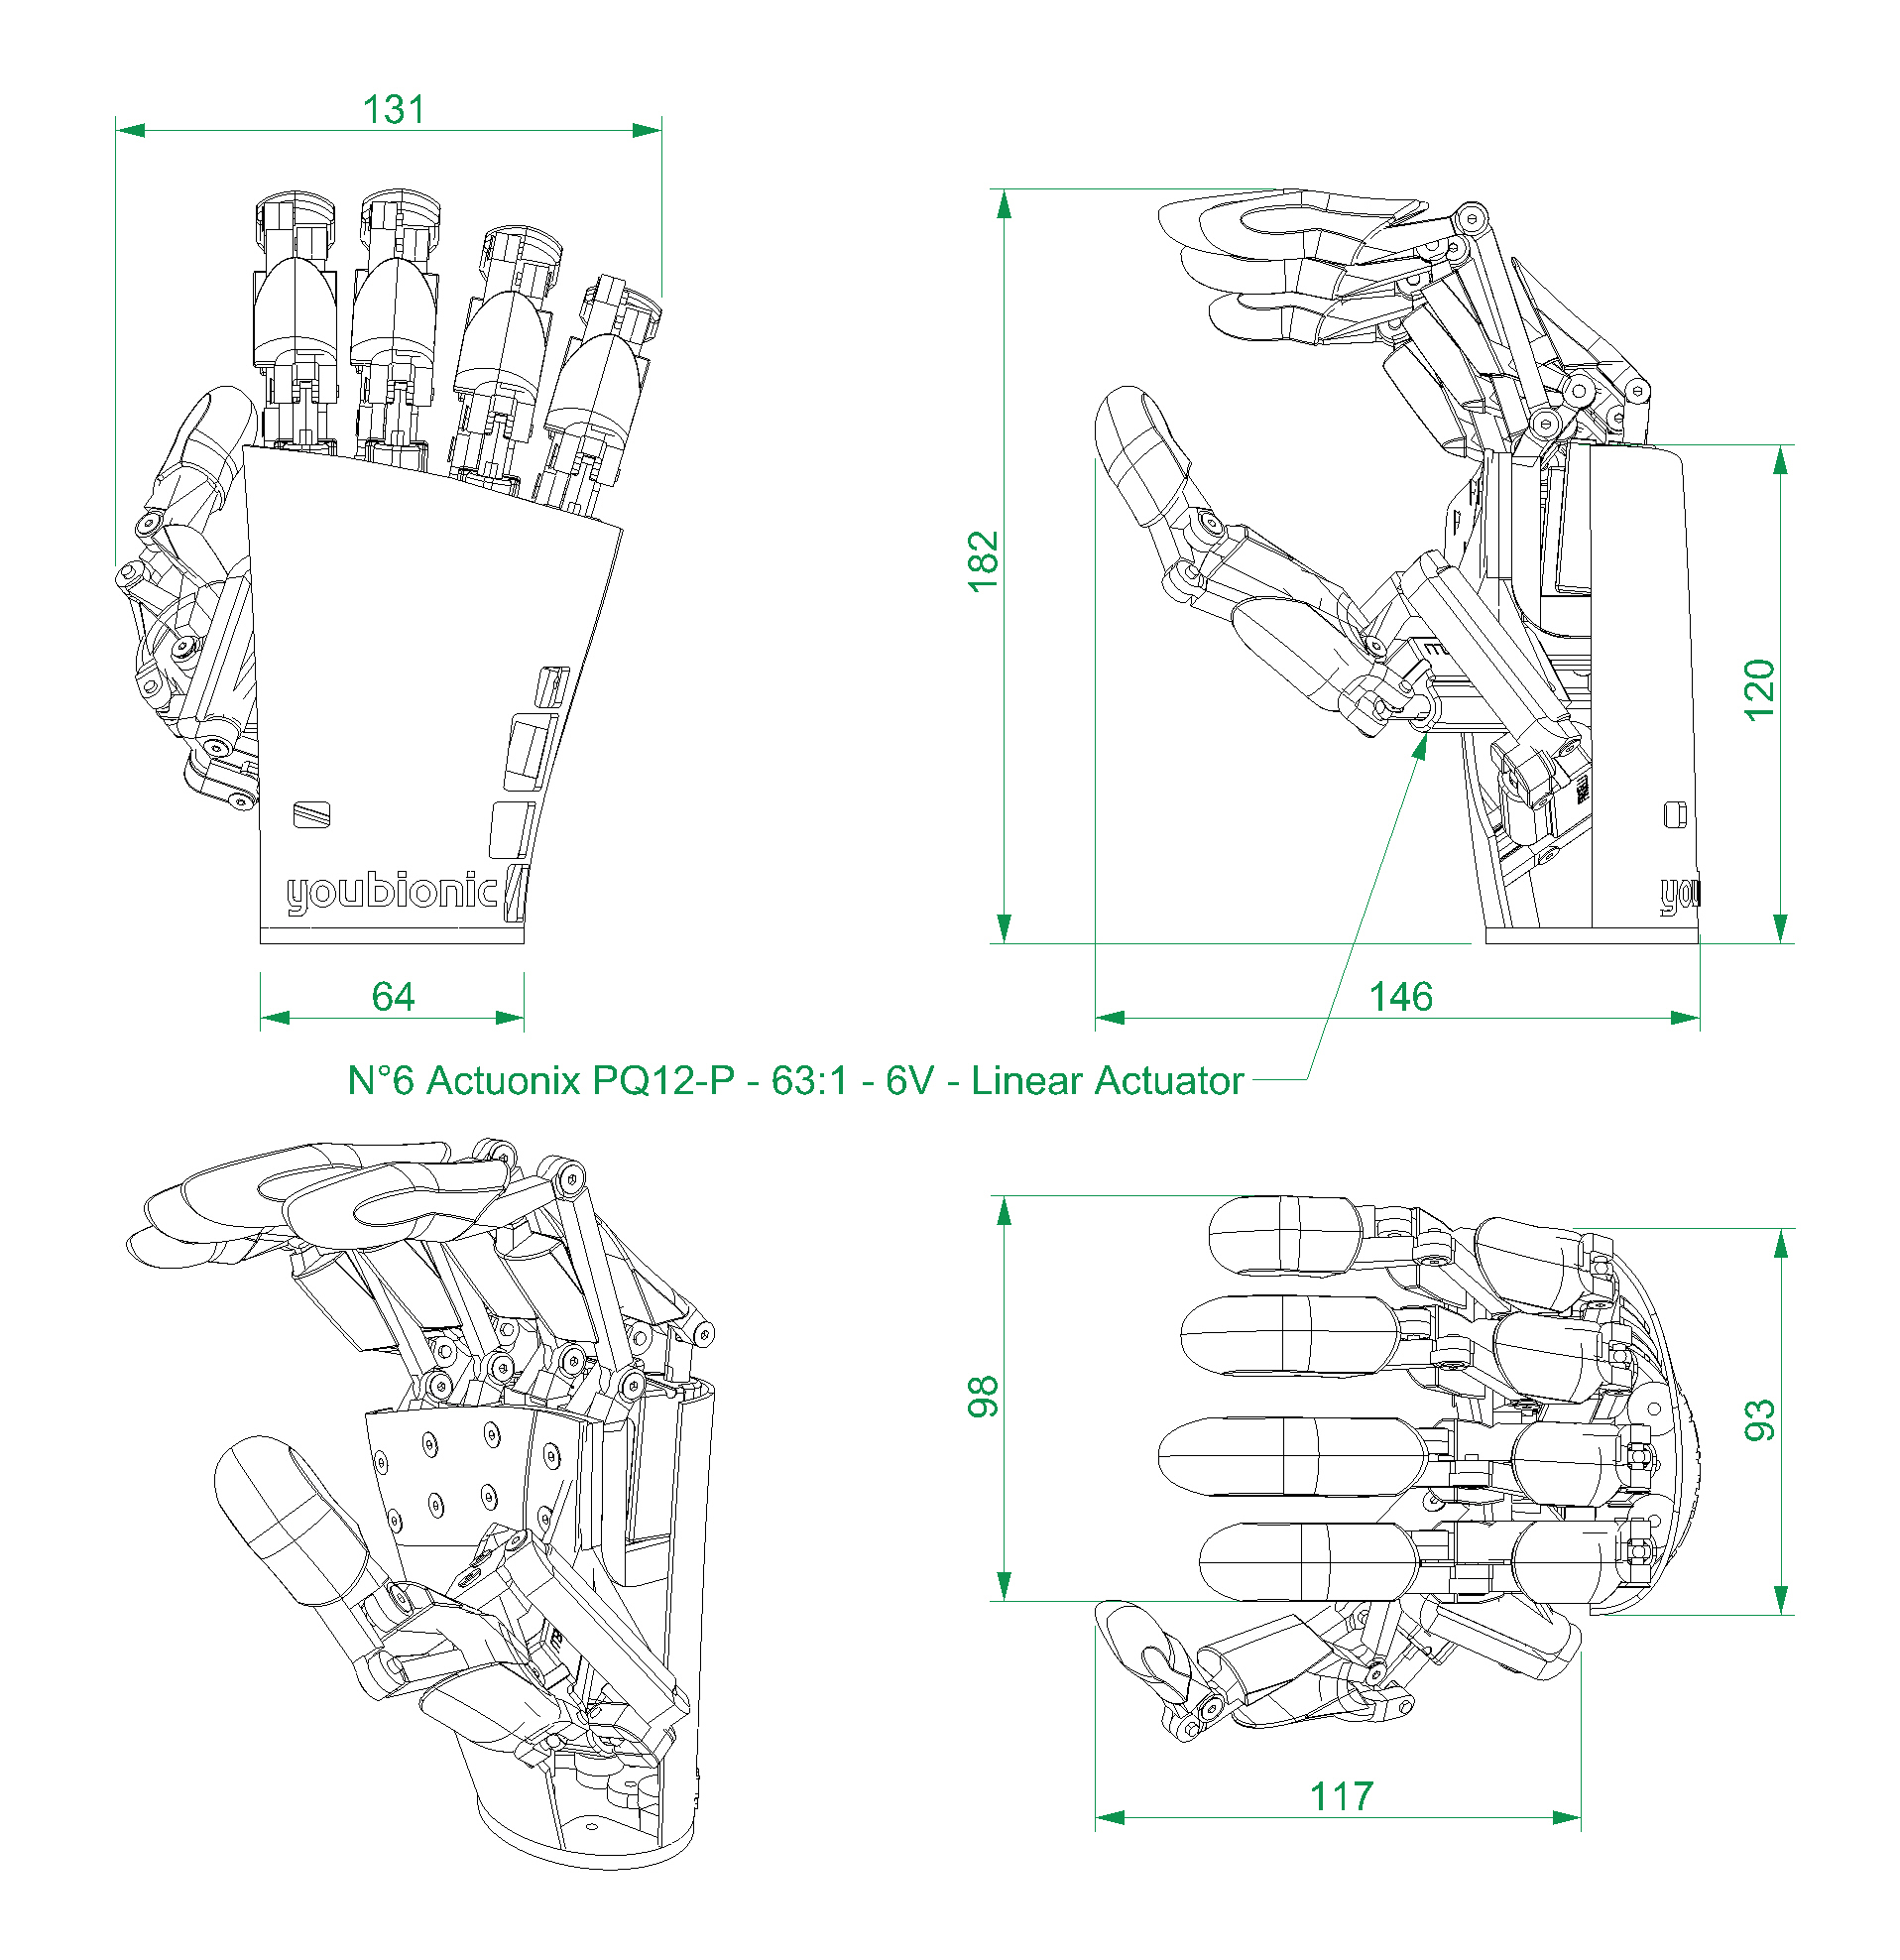
\includegraphics[scale=0.20]{./image/Youbionic-Hand-Technical-Drawing.jpg}
\caption{Youbionic Hand. Převzato z \cite{youBionPic}.}
\label{fig:section-search}

\end{figure}


\begin{figure}[H]
\centering
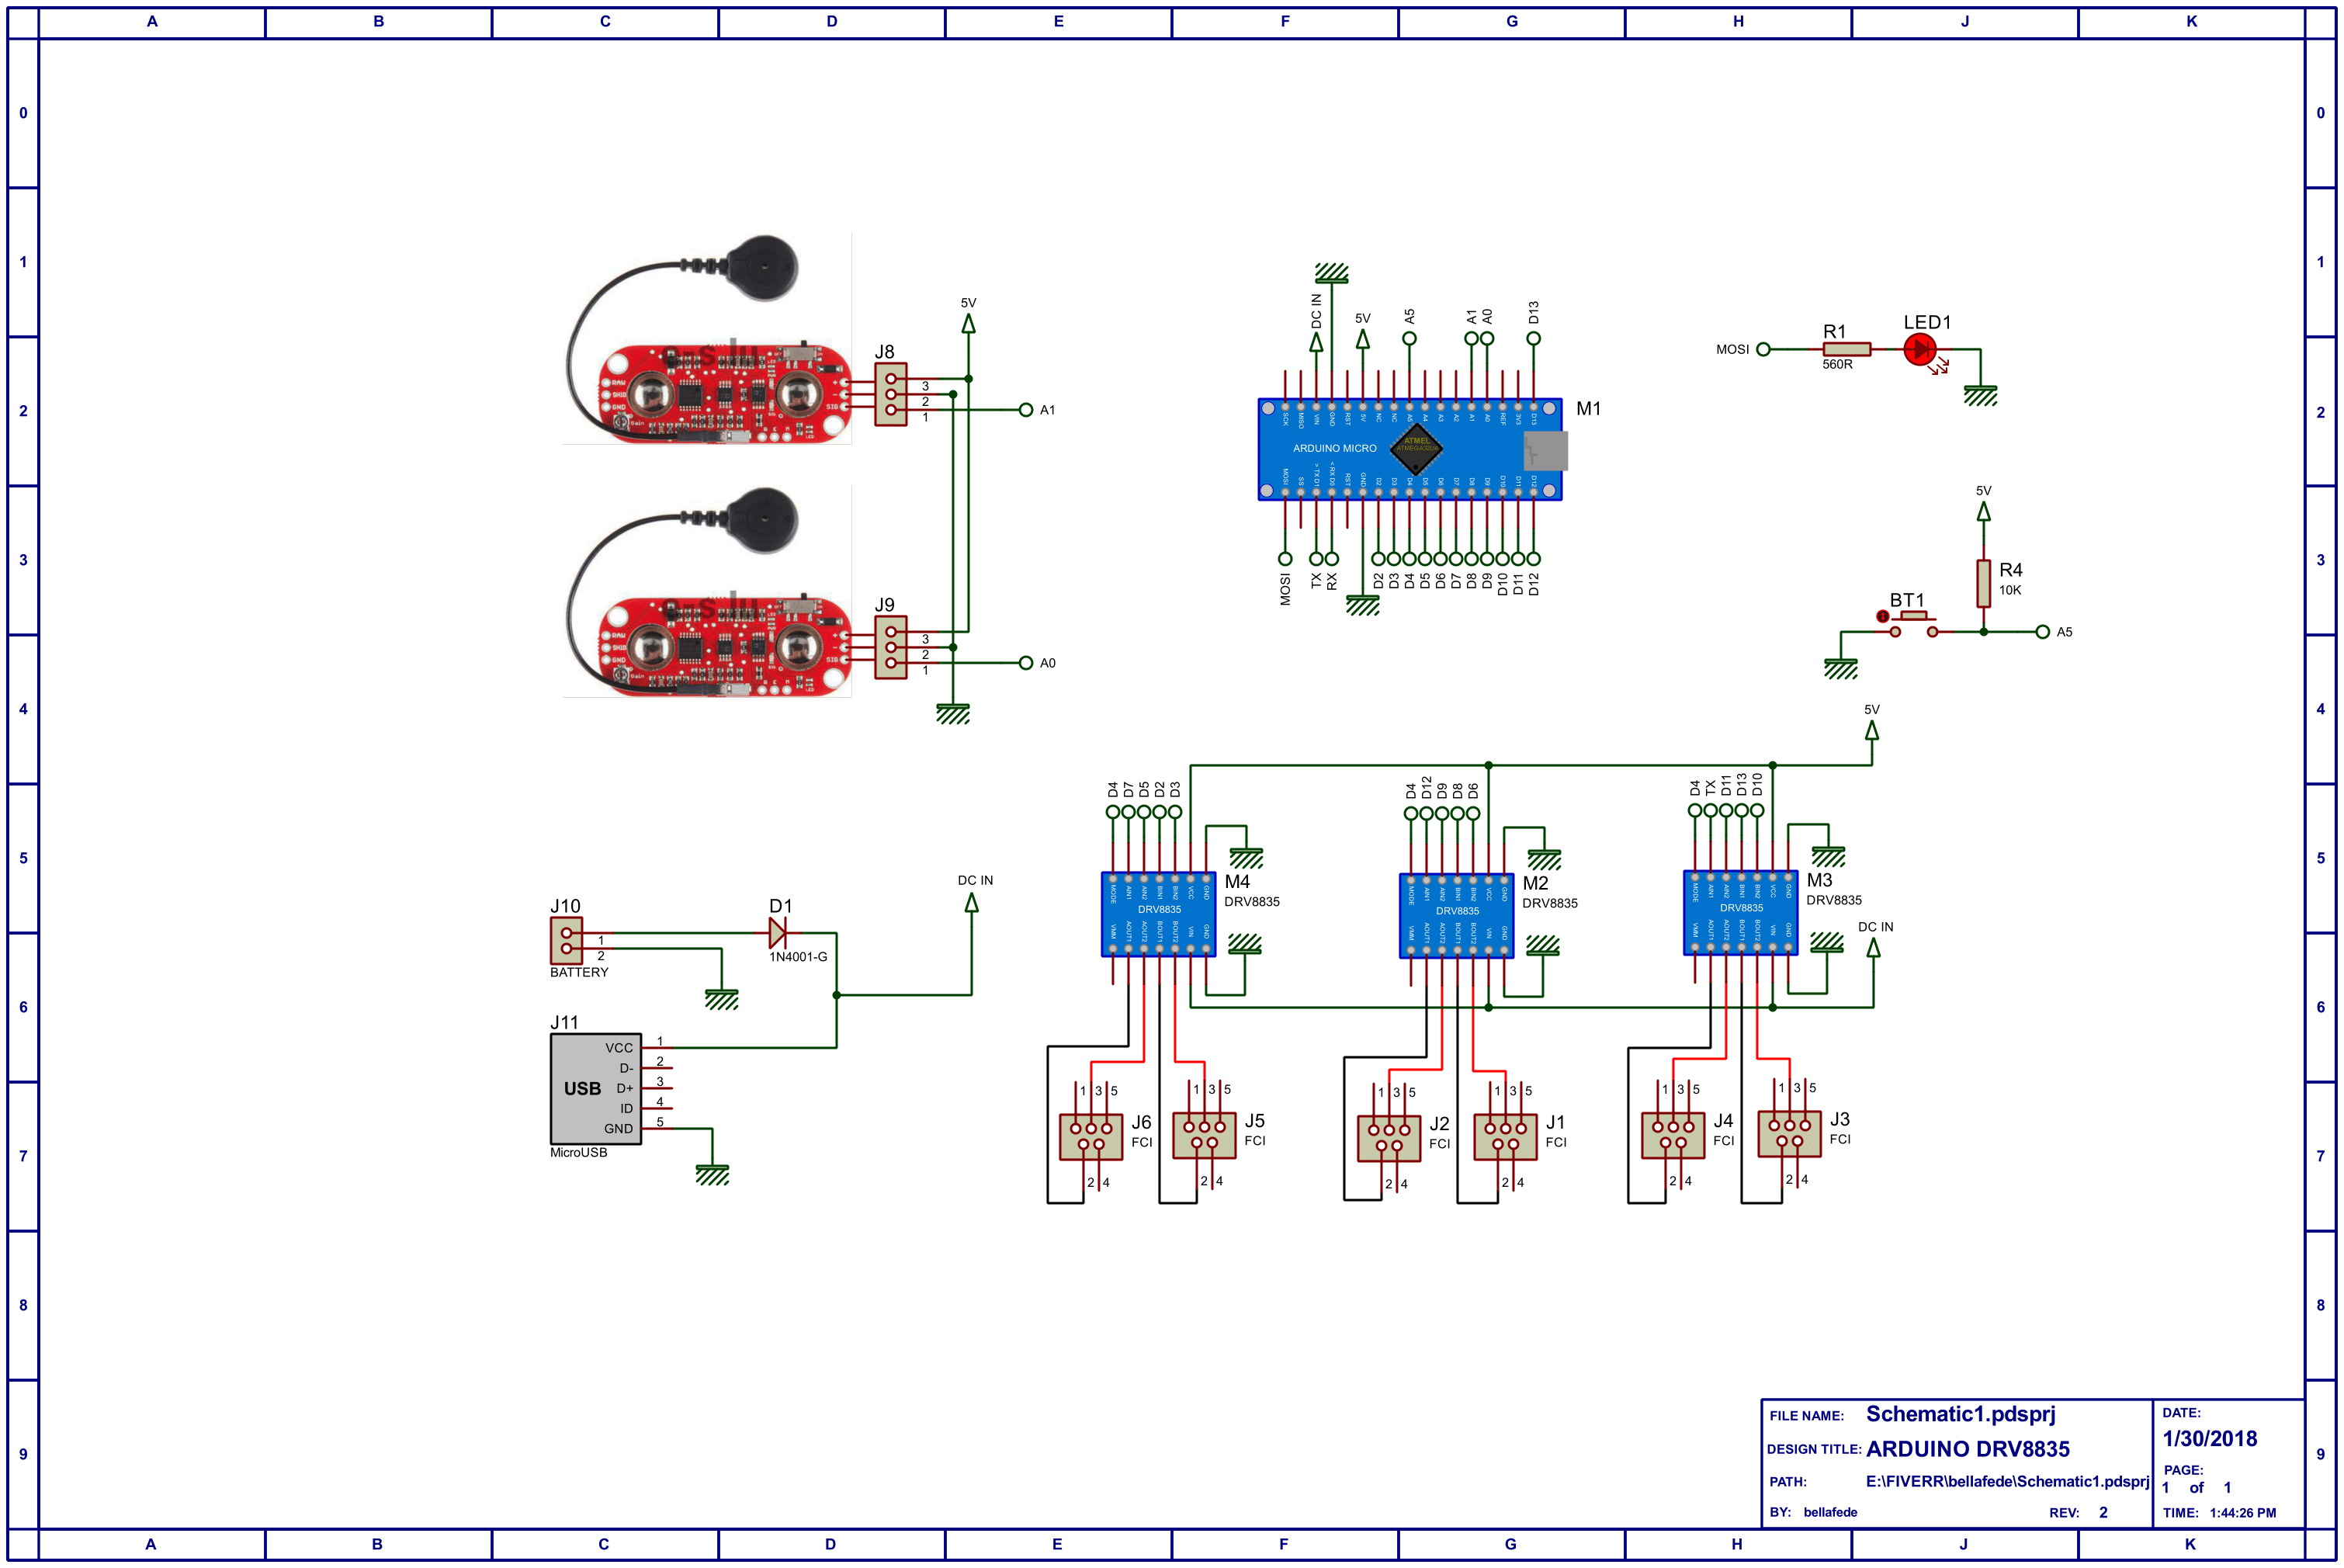
\includegraphics[scale=0.16, angle=90]{./image/YoubionicHandschematic.png}
\caption{Originální schéma zapojení. Převzato z \cite{youBionPic}.}
\label{fig:schema1}

\end{figure}



\subsection{Komponenty}
\label{subsec:Komp}

Tato podkapitola podrobně popisuje hlavní součásti projektu YouBionic Hand, jejich možnosti, vlastnosti a funkce v modelu. 

Hlavní řídicí jednotkou projektu je Arduino Micro, které je k dispozici pro programování. Servomotory které provádí fyzické pohyby rukou jsou připojeny k hlavnímu ovladači. Servomotory jsou připojeny k Arduino prostřednictvím dvoumotorových budičů, které umožňují řídit servomotory. Všechny jednotky modelu jsou připojena k jedné desce, k dispozici je pouze port USB pro programování Arduino a několik výstupních pinů pro připojení externích senzorů. To znamená, že jakékoli změny v původním schématu budou vyžadovat pájení součástí a změny v pouzdru zařízení.


\subsubsection{Arduino Micro}

Arduino je otevřená elektronická platforma. Výhodou platformy je flexibilní software a hardware Arduino, díky kterému je platforma jednoduché konfigurovatelná pro různé projekty. Základním principem zařízení je zpracování vstupních signálů (např. tlakový senzor, tlačítko, atd.).  Deska vstupů je pak schopná zpracovávat a ovládat různé výstupy (rozsvícení LED, spuštění motoru, zobrazení textu na obrazovku, atd.). K programování desek Arduino se používá software Arduino IDE (Vývojové prostředí) (Obrazek \ref{fig:ard-ide}). Programovacím jazykem pro desky Arduino je Wiring, postavený na C a C++. Software je k dispozici na adrese \textit{arduino.cc}. Programy se zapisují na desku pomocí kabelu USB, přes který je deska připojena k počítači. 


\begin{figure}[H]
\centering
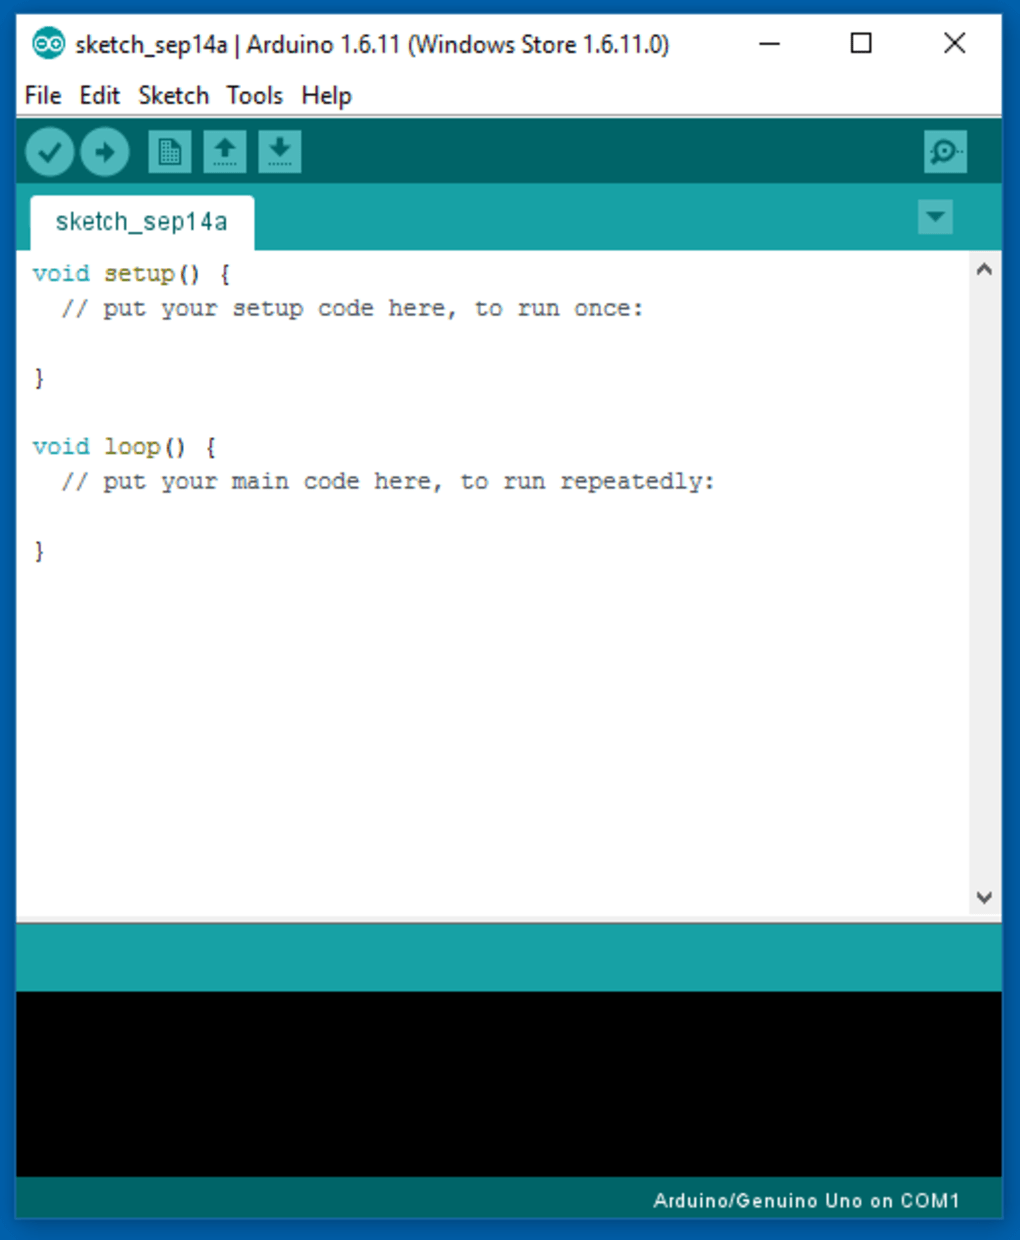
\includegraphics[scale=0.2]{./image/arduino-ide-screenshot.png}
\caption{Arduino IDE}
\label{fig:ard-ide}

\end{figure}


V modelu robotické ruky byl použit ovladač Arduino Micro. \quoting{Arduino Micro obsahuje 20 digitálních I/O pinů (z nichž 7 je možné použít jako PWM (Pulzně Šířková Modulace) výstup a 12 jako analogový vstup), 16MHz krystalový oscilátor, micro USB konektor, ICSP (In-Circuit Serial Programming) čtečku a resetovací tlačítko}\cite{ardMicr}. V Tabulce \ref{tab:ArdMicr} jsou uvedeny specifikace desky Arduino Micro.


\begin{table}[!htbp]\centering
\caption{Technické informace}
\label{tab:ArdMicr}
\begin{tabular}{|l|c|}
 \hline
Mikroprocesor & ATmega32U4  \\ \hline
Provozní napětí (logická úroveň) & 5 V  \\ \hline
Vstupní napětí (doporučeno) & 7-12 V \\ \hline
Vstupní napětí (maximální limit) & 6-20 V \\ \hline
Počet digitálních I/O pinů) & 20 pinů, z toho 7 s PWM \\ \hline
Počet analogových vstupů & 12 pinů \\ \hline
Proudové zatížení na 1 pin & 20 mA \\ \hline
Flash paměť & 32 KB \\ \hline
SRAM & 2,5 KB \\ \hline
EEPROM & 1 KB\\ \hline
Rychlost hodin & 16 MHz \\ \hline
\end{tabular}
\end{table}



Arduino Micro (\ref{fig:subArdMic}) je hlavním řídícím mikrokontrolérem  pro celý projekt. Díky malé velikosti zařízení a dostatečnému množství vstupu je tato verze řídicí desky optimálním řešením pro robotickou ruku. Tento ovladač spojuje a řídí všechny části modelu, řídí servomotory a komunikuje s externími jednotkami (senzory, počítač, atd.). V původním projektu Ardino Micro obsahuje několik volných, pristupovatelných pinů, které lze použít k rozšíření funkčnosti modelu.


\begin{figure}[H]
\centering
  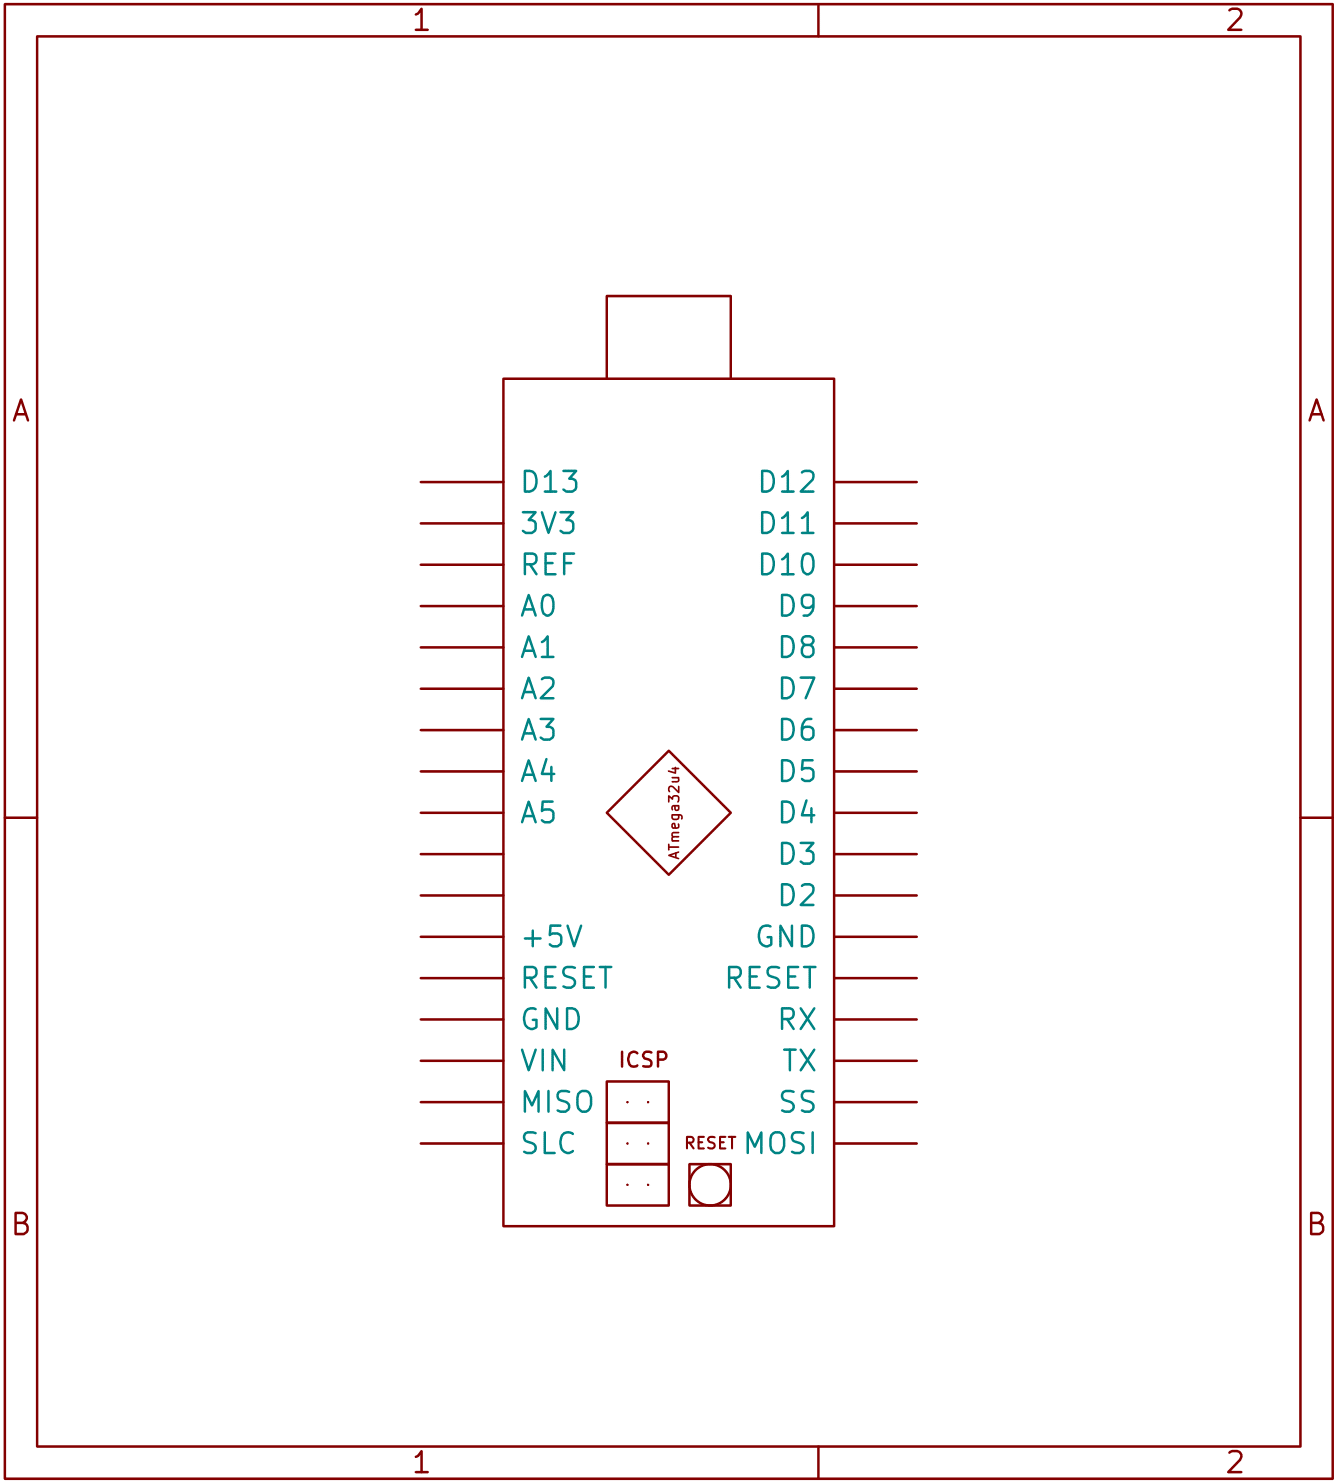
\includegraphics[scale=0.13]{./image/ArdMicro.png}
\caption{Arduino Micro}
  \label{fig:subArdMic}
\end{figure}



\subsubsection{Servomotor}

Pro mechanické pohyby všech pěti prstů robotické ruky se používají servomotory. \quoting{Servo motory slouží pro nastavení určité polohy ovládaného mechanizmu a následné držení v této poloze. Stejnosměrné servo motory se využívají například pro ovládání robotické paže nebo pro nastavení kormidla u leteckých modelů. Jejich hlavní výhodou je malý rozměr a malá hmotnost s relativně velkou silou}\cite{ardServoMan}.


Projekt Youbionic Hand obsahuje šest servopohonů typu PQ12-63-6-P od společnosti Actuonix Motion Devices Inc. Jeden servopohon pohon pro každý prst a jeden pro otáčení palce.


Servopohony PQ12 jsou pohybové přístroje s polohovou zpětnou vazbou pro řízení polohy.  Pohony lze ovládat pomocí stejnosměrného napětí, aby se pohon prodloužil. Změna polarity provede sevření servopohonu.\cite{servo}. Technické vlastnosti servomotoru použitého v modelu jsou uvedeny v Tabulce \ref{tab:servPQ12}. Použité servopohony obsahují potenciometr polohové zpětné vazby. Potenciometr neobsahuje zabudovaný budič, ale poskytuje analogovou zpětnou vazbu. Tuto zpětnou vazbu lze použít k sledování aktuální polohy servopohonu, což je užitečné v modelu robotické ruky pro ovládání polohy prstu. Připojení pinů potenciometru je uvedeno v Tabulce \ref{tab:servPin}. V počátečním provedení není popsaný potenciometr připojen, což neumožňuje řídit stav servomotoru.


\begin{table}[H]

\parbox{.45\linewidth}{
\centering
\caption{Specifikace servopohonu}
\label{tab:servPQ12}
\begin{tabular}{|l|l|}
\hline
Vlastnosti                                                                                         & Hodnota \\ \hline
\begin{tabular}[c]{@{}l@{}}Převodový poměr\end{tabular}					        & 63      \\ \hline
Napětí                                                                                         & 6       \\ \hline
\end{tabular}
}
\hfill
\parbox{.55\linewidth}{
\centering
\caption{Specifikace pinů}
\label{tab:servPin}
\begin{tabular}{|l|l|}
\hline
PIN   & Význam                                         \\ \hline
Pin 1 & \begin{tabular}[c]{@{}l@{}}Zpětná vazba potenciometru \\ negativní referenční kolejnice \end{tabular} \\ \hline
Pin 2 & Napájení pohonu                           \\ \hline
Pin 3 & Napájení pohonu                           \\ \hline
Pin 4 & \begin{tabular}[c]{@{}l@{}}Zpětná vazba potenciometru \\ pozitivní referenční kolejnice \end{tabular}   \\ \hline
Pin 5 & Potenciometr zpětné vazby                 \\ \hline
\end{tabular}
}
\end{table}


\subsubsection{Budiče pro motory}


Servomotory použité v modelu neobsahují integrované ovladače. Projekt proto používá ovladače DRV8835 od společnosti Texas Instruments. Ke každému regulátoru jsou připojeny dva pohony. V rámce projektů používané řídící rozhraní ovladače je PHASE/ENABLE. Rozhraní je zvoleno prostřednictvím pinu Mode. V tomto rozhraní jeden pin je určený  pro směr otáčení (AIN1/BIN1) a druhý pin pro rychlost (AIN2/BIN2)\cite{drvBr}.  Pro ovládání dvou servomotorů jsou ke každému regulátoru připojeny čtyři výstupní signály Arduino (dva pro každý motor). Tato konfigurace řídicí jednotky servomotoru neobsahuje přiřazenou zpětnou vazbu z pohonu, tj. v původním modelu není možné nastavit servomotor (nebo prst robotické ruky) do konkrétní polohy.


\subsection{Programové řešení}
\label{subsec:progRes}


Projekt YouBionic Hand obsahuje základní řešení pro řízení modelu pomocí svalového senzoru MyoWare.


Svalový senzor měří aktivaci svalů elektrickým potenciálem. Senzor MyoWare má navíc analogový výstup v rozsahu 0-1023\cite{MusSensDoc}. Díky této funkci je tento senzor snadno kompatibilní s Arduino. Připojením tohoto senzoru k Arduino v ruce můžeme zkontrolovat původní řešení pro ovládání modelu. Robotická ruka reaguje na stisknutí a uvolnění ruky uživatele. Na základě pohybu, všechny prsty v modelu se otevírají/zavírají. V tomto řešení není implementováno ovládání různých prstů zvlášť a otáčení palce.


Výrobce poskytuje kód pro své rešení. Je to jediná softwarová část projektů, která v době psaní práce je k dispozici. Softwarovou součástí projektu je skript napsaný pro Arduino Micro. Můžeme analyzovat tuto část projektu, testováním původního programu.


Arduino řídí servomotory prostřednictvím výstupních signálů připojených k budičům servopohonů. K ovládání každého servomotoru se používají dva výstupní signály. První označuje směr otáčení pohonu. Druhý signál nastavuje rychlost otáčení. Počáteční konfigurace pinů jsou uvedeny v Tabulce \ref{tab:VarDescr}. V kódu také se konfigurujou budiče servopohonů. Budiče jsou nastaveny do režimu PHASE/ENABLE. Pro ovládání dvou pohonů jedním komponentem. Pro řízení motorů v kódu aplikace jsou použity funkce z Ukázky \ref{code:HandCont}, kde \textit{direction} je směr motoru (LOW - otevírání, HIGH - zavírání), \textit{speed} je rychlost otáčení.


\begin{table}[H]
\centering
\catcode`\-=12
\caption{Konfigurace pinů}
\label{tab:VarDescr}
\begin{tabular}{|l|c|c|}
\hline
\textbf{Proměnná} & \textbf{PIN} & \textbf{Ovládaný prst}           \\ \hline \hline
pinDirA           & 2            & \multirow{2}{*}{Ukazováč}        \\ \cline{1-2}
pinPwmA           & 3            &                                  \\ \hline
pinDirB           & 7            & \multirow{2}{*}{Prostředník}     \\ \cline{1-2}
pinPwmB           & 5            &                                  \\ \hline
pinDirC           & 8            & \multirow{2}{*}{Prsteník}        \\ \cline{1-2}
pinPwmC           & 6            &                                  \\ \hline
pinDirD           & 12           & \multirow{2}{*}{Malíček}         \\ \cline{1-2}
pinPwmD           & 9            &                                  \\ \hline
pinDirE           & 13           & \multirow{2}{*}{Palec}           \\ \cline{1-2}
pinPwmE           & 10           &                                  \\ \hline
pinDirF           & 1            & \multirow{2}{*}{Palcové otáčení} \\ \cline{1-2}
pinPwmF           & 11           &                                  \\ \hline
\end{tabular}
\end{table}

\newpage

\begin{lstlisting}[caption={Funkce pro ovládání motoru},label={code:HandCont}]

 digitalWrite( pinDir,direction );
 analogWrite( pinPwm,speed ); 
 
\end{lstlisting}



Procesy otevírání a zavírání celé ruky jsou řízeny pomocí vstupního signálu ze svalového senzorů. Svalový senzor připojen na pin A1 a čtení signálů z tohoto pinu realizované pomocí funkce: \texttt{analogRead(pin)}. Pro správné zpracování signálů se provádí fáze kalibrace senzoru, fáze kalibrace vyžaduje od uživatele používat svaly, na které je senzor přiřazen. Fáze kalibrace trvá 10 vteřin, výsledkem této fáze jsou minimální a maximální hodnoty naměřené snímačem. Hlavní funkcí programu je cyklus, ve kterém aplikace sleduje aktivitu svalů uživatele a na základě výstupu snímače provádí pro otevření a zavření robotické ruky.


YouBionic Hand nemá knihovnu ani dokumentaci popisující funkci pro ovládání modelu. Analyzovány v této podkapitole program je částečně popsán pomocí komentářů. Ten program je jediné softwarové řešení, které společnost YouBionic poskytuje pro svůj výrobek. Toto řešení je použitelný pro testování možností modelu a části kódu mohou být použity pro návrh softwarového vybavení v rámci práce.


\section{Lidská ruka}
\label{sec:hand}
Předmětem bakalářské práce je robotická ruka vytvořená ve tvaru lidské ruky. Mechanické pohyby modelu proto musí odpovídat pohybu lidské ruky. Jedním z cílů práce je implementace zachycení objektů. Po prostudování způsobů uchopení předmětu lidskou rukou můžeme realizovat podobný pohyb v modelu. Na základě těchto informací a charakteristik modelu můžeme zjistit, jaké formy pohybu lze v práci použít.


Metody zachycení a držení objektu jsou rozděleny do tří hlavních skupin: zachycení(\ref{fig:simplGrip}) ,zachycení pomocí gravitace(\ref{fig:gravGrip}), zachycení spolu s akcí(\ref{fig:actionGrip}). V této části již můžeme říci, že konstrukce robotické ruky použité v práci není vhodná pro třetí skupinu zachycení. Protože zachycení s akcí vyžaduje použití svalů prstů a puky, které nejsou v modelu implementovány. Například otáčení prstu a pohyb pouze části prstu. Druhá skupina zachycení nevyžaduje složité řešení pro ovládání modelu, v podstatě jde o podporu objektu. Proto v této práci budeme věnovat pozornost první skupině. Skupina zachycení je rozdělena do tří podskupin\cite{PhysJoin}:

\begin{itemize}
\item prstové - zachycení je provedeno pouze pomocí prstů.
\item dlaňové - při uchopení se používají dlaň a prsty.
\item středové -  úchyty vytvářejí symetrii kolem podélné osy, která se obvykle shoduje s osou předloktí.
\end{itemize}


Každá z těchto podskupin obsahuje úchop, který lze realizovat v použité robotcké ruce. Návrh a implementace těchto technik zachycení je cílem praktické části práce.

 
 
 \begin{figure}[H]
\centering
\begin{subfigure}{.3\textwidth}
  \centering
  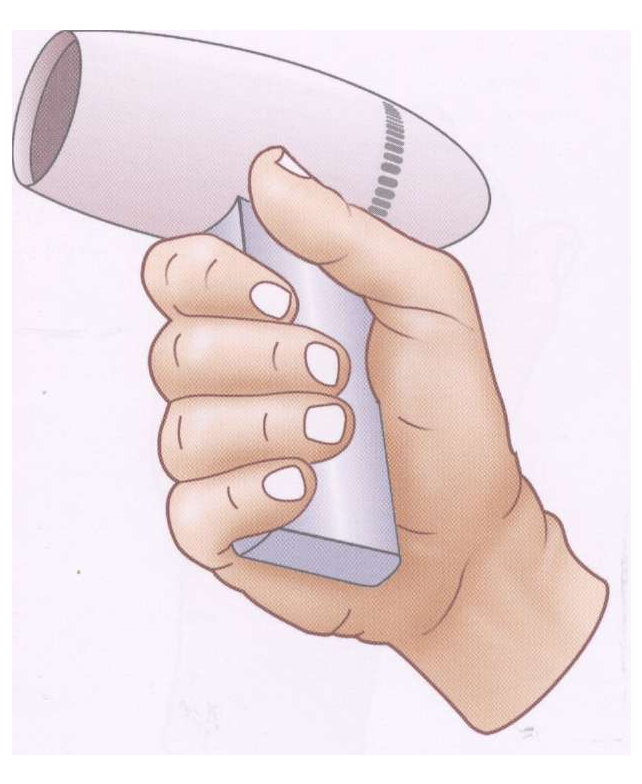
\includegraphics[width=.6\linewidth]{./image/simplGrip.png}
  \caption{Zachycení. Převzato z \cite{PhysJoin}.}
  \label{fig:simplGrip}
\end{subfigure}
\begin{subfigure}{.5\textwidth}
  \centering
  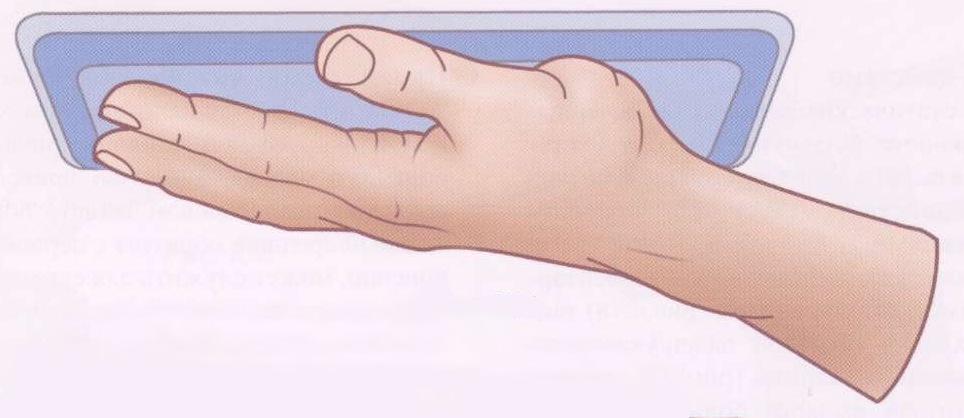
\includegraphics[width=.7\linewidth]{./image/gravGrip.png}
  \caption{Zachycení pomocí gravitace. Převzato z \cite{PhysJoin}.}
  \label{fig:gravGrip}
\end{subfigure}
\label{fig:test}
\begin{subfigure}{.3\textwidth}
  \centering
  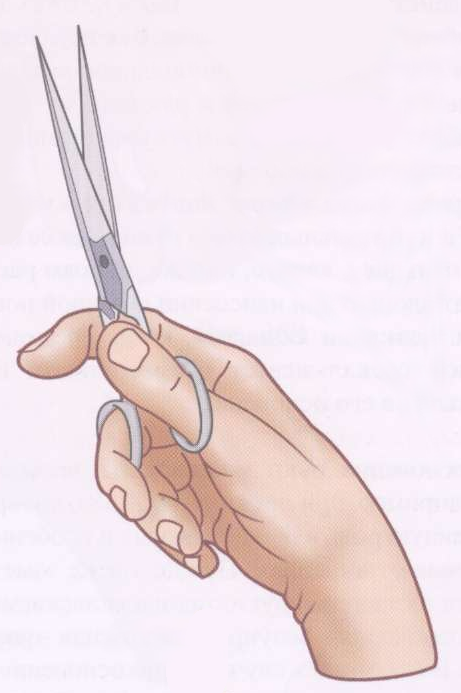
\includegraphics[width=.6\linewidth]{./image/actionGrip.png}
  \caption{Zachycení spolu s akcí. Převzato z \cite{PhysJoin}.}
  \label{fig:actionGrip}
\end{subfigure}
\label{fig:test}

\end{figure}
 

 \begin{figure}[H]
\centering
\begin{subfigure}{.4\textwidth}
  \centering
  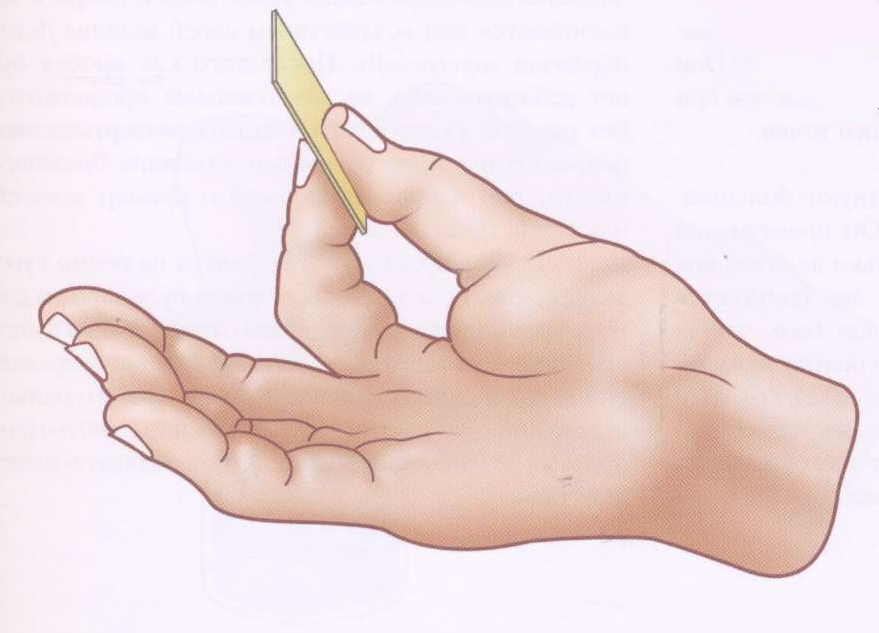
\includegraphics[width=.6\linewidth]{./image/fingGrip.png}
  \caption{Prstové zachycení. Převzato z \cite{PhysJoin}.}
  \label{fig:fingGrip}
\end{subfigure}
\begin{subfigure}{.4\textwidth}
  \centering
  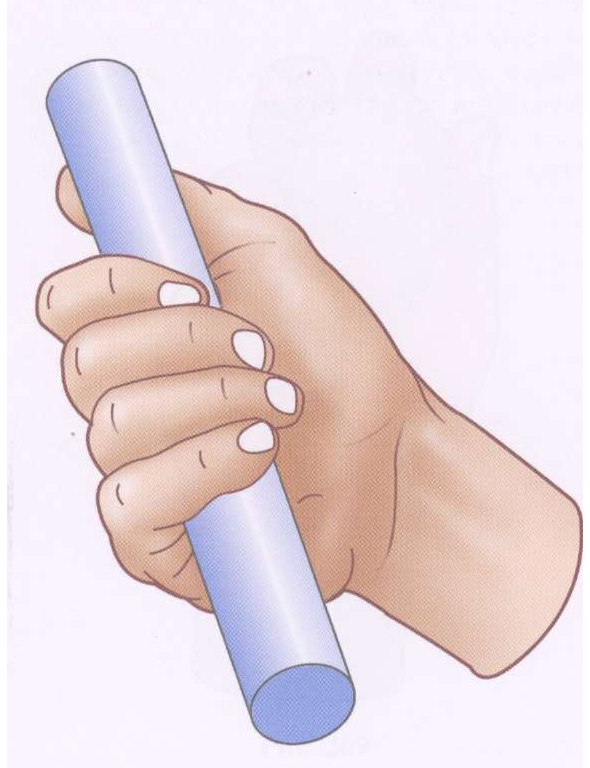
\includegraphics[width=.6\linewidth]{./image/dlanGrip.png}
  \caption{Dlaňové zachycení. Převzato z \cite{PhysJoin}.}
  \label{fig:dlanGrip}
\end{subfigure}
\label{fig:test}
\begin{subfigure}{.4\textwidth}
  \centering
  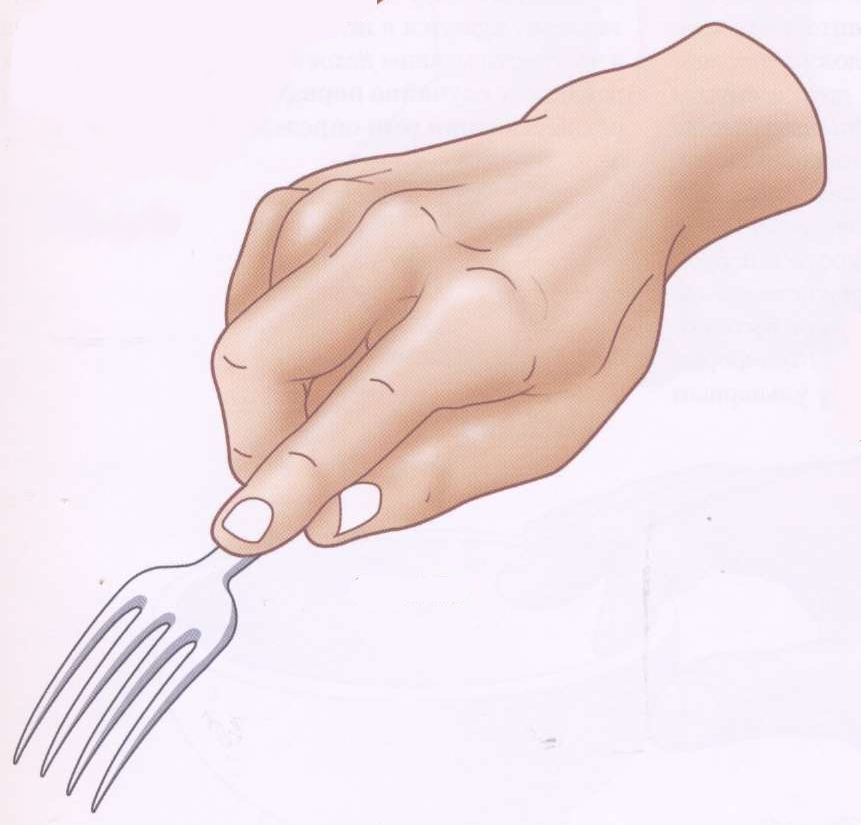
\includegraphics[width=.6\linewidth]{./image/centSimpGrip.png}
  \caption{Středové zachycení. Převzato z \cite{PhysJoin}.}
  \label{fig:centSimpGrip}
\end{subfigure}
\label{fig:test}

\end{figure} 
 
 

\chapter{Testování možností modelu}
\label{ch:test}

V této kapitole otestujeme model robotické ruky Youbionic. Musíme identifikovat objekty, které model dokáže zachytit a držet. Pro testování provedeme změny v původním  řešení řízení modelu od výrobce. Změníme princip ovládání otevírání a zavírání ruky, pomocí svalového senzoru namísto svalového senzoru bude model cyklicky otevírat a zavírat ruku. Pro různé typy objektů jsou určeny různé počáteční stavy otevřené ruky pro implementaci různých typů uchopení. Tyto typy úchopů jsou popsány v předchozí kapitole. Program pro testování je v elektronické příloze k práci. Vybereme osm předmětů různých tvarů, materiálů a hmotností. Vybrané objekty umožňují testovat různé typy zachycení a lidé je také denně používají. Všechny položky váží méně než 0,6 kg pro testování, aniž by došlo k poškození modelu. Výsledky testů jsou podrobně popsány v Tabulce \ref{tab:test}.


Výsledky zkoušek ukazují, že model je vhodný pro zachycení válcových předmětů a není vhodný pro práci s malými předměty. Ve robotické ruce vybrané pro tuto práci není pohyb určité části prstu a rotace zamýšlen. Model umožňuje pohyb pouze celého prstu. Tato omezení znemožňují přesnou práci(např. psaní), ale model nedokáže s přesností uchopit malé objekty. 



\begin{sidewaystable}[]
\caption{Výsledky testů}
\label{tab:test}
\begin{tabular}{|l|l|l|l|l|l|}
\hline
Předmět        & Popis                                                                        & \begin{tabular}[c]{@{}l@{}}Velikosti\\ , cm\end{tabular} & \begin{tabular}[c]{@{}l@{}}Hmotnost\\ , g\end{tabular} & \begin{tabular}[c]{@{}l@{}}Způsob \\ zachycení\end{tabular} & Výsledek                                                                                                                                                                                         \\ \hline
Tužka          & \multicolumn{1}{c|}{-}                                                       & 16 x  0,7                                                & 8                                                      & prstové/středové                                            & \begin{tabular}[c]{@{}l@{}}Ruka může držet tužku mezi \\ palcem a ukazováčem. A nebo \\ uchopit tužku, aby byla vhodná \\ pro psaní. Nicméně, síla stisku \\ není vhodná pro psaní.\end{tabular} \\ \hline
Sklenici       & \begin{tabular}[c]{@{}l@{}}válcové \\ prázdné sklo\end{tabular}              & 14 x 9                                                   & 240                                                    & dlaňové                                                     & \begin{tabular}[c]{@{}l@{}}Ruka je schopna sklenici zachytit \\ a držet.\end{tabular}                                                                                                            \\ \hline
Hrnek          & \begin{tabular}[c]{@{}l@{}}prázdný \\ hrnek\end{tabular}                     & 10 x 8                                                   & 160                                                    & prstové                                                     & Ruka může hrnek držet za rukojeť.                                                                                                                                                                \\ \hline
Kniha          & \begin{tabular}[c]{@{}l@{}}vázaná \\ kniha\end{tabular}                      & 19 x 13 x 2                                              & 350                                                    & prstové                                                     & \begin{tabular}[c]{@{}l@{}}Ruka nemůže manipulovat se \\ stránkami knihy. Ale může \\ chytit a držet celou knihu.\end{tabular}                                                                   \\ \hline
Kladivo        & \multicolumn{1}{c|}{-}                                                       & 25 x 3                                                   & 470                                                    & dlaňové                                                     & \begin{tabular}[c]{@{}l@{}}Ruka může uchopit kladivo \\ za rukojeť, ale síla uchopení \\ je pro pevné uchopení \\ nedostatečná. Rukojeť \\ kladiva vyklouzla z ruky.\end{tabular}                \\ \hline
Plastová láhev & \begin{tabular}[c]{@{}l@{}}plná plastová \\ láhev 0,5l\end{tabular}          & 23 x 8                                                   & 522                                                    & dlaňové                                                     & Ruka může chytit láhev a držet ji                                                                                                                                                                \\ \hline
Míč            & \begin{tabular}[c]{@{}l@{}}gumový \\ míč\end{tabular}                        & 9 x 9 x 9                                                & 41                                                     & dlaňové                                                     & \begin{tabular}[c]{@{}l@{}}Ruka dokáže uchopit míč \\ nebo jiný kulový předmět.\end{tabular}                                                                                                     \\ \hline
Papír          & \begin{tabular}[c]{@{}l@{}}několikrát \\ složený \\ list papíru\end{tabular} & 10 x 5                                                   & 5                                                      & prstové                                                     & \begin{tabular}[c]{@{}l@{}}Ruka může držet papír \\ mezi palcem a ukazováčkem.\end{tabular}                                                                                                      \\ \hline
\end{tabular}
\end{sidewaystable}


\chapter{Analýza a návrh}

Tato kapitola je věnována analýze a vývoji řešení. V kapitola jsou popsané technologie zvolené pro dosažení cílů této prace a jsou navržené změny v modelu a řešení pro ovládání robotické ruky. Jsou navržena funkčnost aplikace pro demonstraci možnosti robotické ruky a uživatelské rozhraní této aplikace.

\section{Polohy prstů robotické ruky}

Hlavním cílem práce je ovládání robotické ruky. Pro co nejpřesnější ovládání modelu potřebujeme vědět aktuální polohu všech prstů. Pro tyto účely, PQ12 pohony použité v modelu mají potenciometr zpětné vazby. Servopohony nemají vestavěné budiče a potenciometr zpětné vazby nebyl použit v původním modelu. Ze studie v teoretické části práce, dokumentaci pohonu, víme, že výstup potenciometru je umístěn na PIN1 servopohonu a je analogový signál. Můžeme tento signál připojit k Arduino a sledovat výstupní napětí potenciometrů. Výstupní napětí potenciometrů je úměrné poloze pohonu, ke kterému je připojeno. Poloha pohonu v modelu manipulátoru odpovídá poloze prstu, který řídí servomotor\cite{PotenPosit}.


Prvním praktickým úkolem práce je připojit zpětnou vazbu servopohonů k modelu, aby bylo možné řídit pohony v závislosti na jejich poloze. Robotická ruka má šest servopohonů, takže potřebujeme šest volných kontaktů na ovládací desce. Arduino Micro, který řídí model, neobsahuje dostatek volných pinů, které lze použít k připojení zpětné vazby z servopohonu. Zvolené řešení je přidat další ovládací prvek a nastavit spojení mezi původní deskou a deskou periferní. Toto řešení bylo zvoleno z několika důvodů:

\begin{itemize}
 \item toto řešení vyžaduje minimální změny v konstrukce původního modelu
 \item nedostatek volných pinů na původní desce
 \item možnost přidání dalších senzorů a jiných vstupů a výstupů do celého projektu
\end{itemize}
 
Pro tyto účely byla zvolena deska \uv{DM Pro Mini Strong}, která je plně kompatibilní s Arduino. Díky kompatibilitě a malé konstrukce tato deska je optimálním řešením pro integrace do modelu a splnění cílů práce. 


Na Obrázku \ref{fig:DesHandSch} je navržen nový diagram modelu. Výstupy potenciometru servomotoru jsou připojeny k desce Pro Mini Strong, která komunikuje s Arduino Micro. Arduino Micro na základě zpětné vazby potenciometru nastavuje polohu servopohonů.

\begin{figure}[H]
\centering
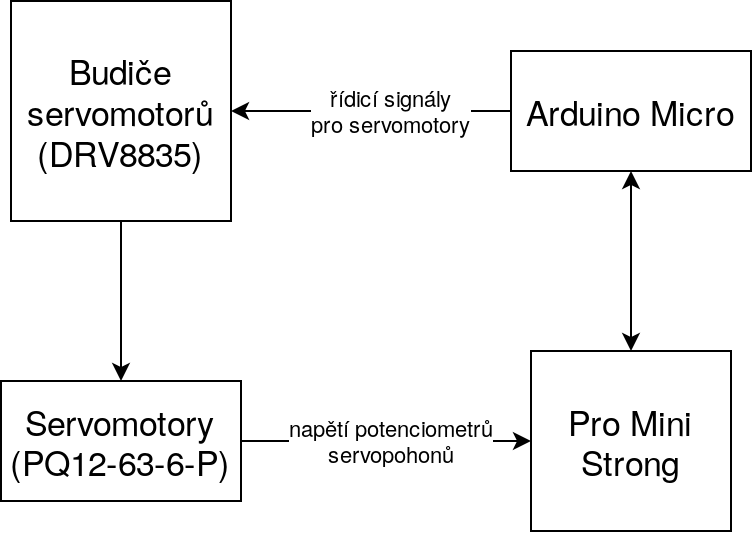
\includegraphics[scale=0.32]{./image/DesigneHandScheme.png}
\caption{Komunikace komponent robotické ruky}
\label{fig:DesHandSch}
\end{figure}


\section{Komunikace mezi deskami Arduino}

Externí deska Pro Mini Strong, ke které připojime výstupy servopohonů, je použita v navrhovaném řešení ovládání robotické ruky. Pro přístup k těmto výstupům musíme připojit vybranou desku k hlavní řídicí desce modelu (Arduino micro).


Existuje několik různých řešení pro komunikaci mezi deskami Arduino. Většina komunikačních řešení (např. Standard Serial communication, I2C serial communication) používá výstupní piny Arduino, které jsou již v původním modelu použity nebo jsou nepřístupné. Zvoleným řešením je komunikace prostřednictvím SPI (Serial Peripheral Interface). SPI je synchronní sériový datový protokol používaný mikrokontroléry pro komunikaci s jedním nebo více periferními zařízeními rychlé na krátké vzdálenosti. V původním návrhu modelu jsou výstupy pro komunikaci přes SPI k dispozici bez jakýchkoli změn v projektu. SPI má linky MISO, MOSI, SS a CLK\cite{spiAtm}.

 \begin{itemize}
  \item MISO (Master in Slave Out) - Slave linka pro odesílání dat do Master.
  \item MOSI (Master Out Slave In) - Master linka pro odesílání dat do periferie.
  \item SCK (Serial Clock) - Hodinové impulsy synchronizující přenos dat generovaný Masterem.
  \item SS (Slave Select) - Master může pomocí teto linky vybrat konkrétní zařízení.
 \end{itemize}

 
Obrázek \ref{fig:SPIClassic} ukazuje standardní schéma připojení přes SPI. Tabulka \ref{tab:SpiPins} ukazuje umístění komunikačních linek SPI na použitých deskách. V navrhovaném řešení jsou pouze dvě zařízení, takže není nutné používat linku SS. Zbývající linky potřebné pro komunikaci mezi deskami jsou umístěny na rozhraní ICSP (Obrázek \ref{fig:ICSP}), které se používá k programování desky prostřednictvím sériové linky. Toto rozhraní je snadno přístupné a přes toto rozhraní bude externí deska poháněná hlavní řídicí jednotkou. Z těchto důvodů byl zvolen navrhovaný způsob připojení.

 
 \begin{figure}[H]
\centering
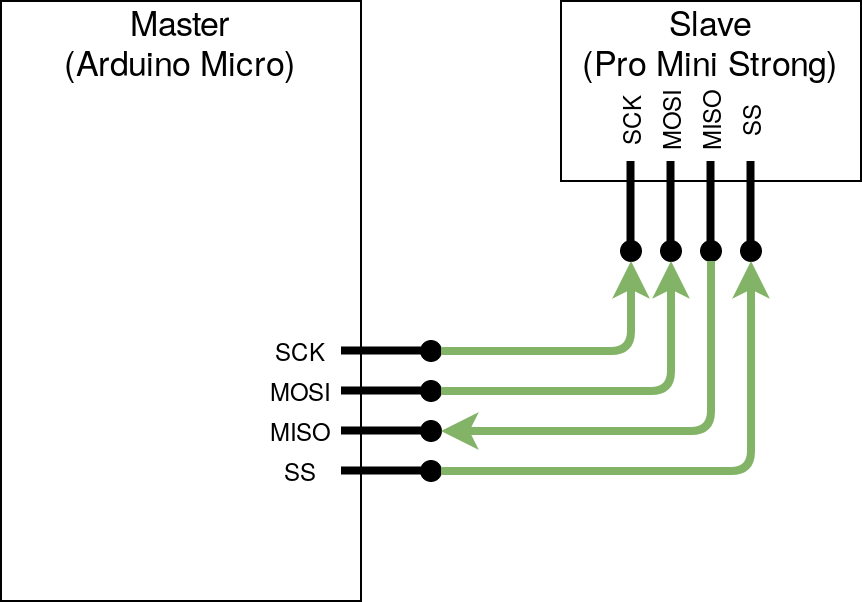
\includegraphics[scale=0.3]{./image/SPIClassic.png}
\caption{SPI komunikace}
\label{fig:SPIClassic}
\end{figure}
 
 \hspace{4cm}
 
\begin{minipage}{\textwidth}
  \begin{minipage}[b]{0.28\textwidth}
    \centering
    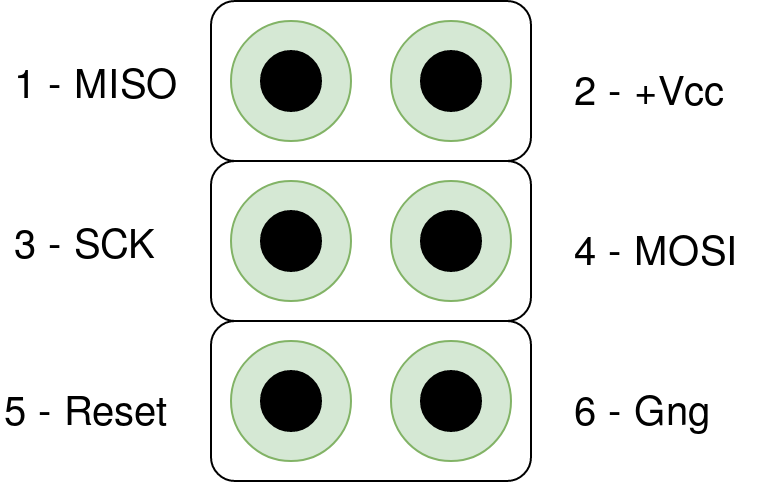
\includegraphics[scale=0.15]{./image/ICSP.png}
    \captionof{figure}{ICSP}
    \label{fig:ICSP}
  \end{minipage}
  \hfill
  \begin{minipage}[b]{0.7\textwidth}
    \centering
    \begin{tabular}{|l|l|l|}
    \hline
    SPI Linka & Arduino Micro & \begin{tabular}[c]{@{}l@{}}DM Pro Mini\\ Strong\end{tabular} \\ \hline
    MOSI      & 10 nebo ICSP-4  & 15 nebo ICSP-4                                                 \\ \hline
    MISO      & 11 nebo ICSP-1  & 16 nebo ICSP-1                                                 \\ \hline
    SCK       & 9 nebo ICSP-3   & 17 nebo ICSP-3                                                 \\ \hline
    SS        & 8             & 14                                                           \\ \hline
  \end{tabular}
      \captionof{table}{Umístění linek SPI}
      \label{tab:SpiPins}
    \end{minipage}
  \end{minipage}

\newpage
 

 
 Pro implementaci komunikace pomocí SPI použijeme knihovnu \texttt{SPI.H} pro Arduino. Arduino Micro bude nastaveno do režimu Master a DM Pro Mini Strong do režimu Slave. Na straně Master můžeme použít funkci \texttt{SPI.transfer (Mastersend)}, jejíž prostřednictvím budeme odesílat data do zařízení Slave a současně vyvolávat přerušení na Slave zařízení. Implementujeme zpracování přerušení tak, aby Slave předal data Masteru na základě získaných dat.
 

\section{Řízení modelu}

Správné řízení modelu robotické je jedním z cílů této práce. Proto je potřeba zvolit řídicí systém, ktrerý bude použit pro ovládání modelu. Řídící systémy jsou rozděleny do dvou obecných kategorií: systémy s otevřenou smyčkou a uzavřenou smyčkou. Rozdíl je v regulační akcí, která odpovídá za výstup systému. Principy těchto systémů jsou popsány v knize \uv{Feedback and control systems}\cite{contrSyst}.

V původním řešení je vztah mezi vstupem a výstupem přímý a není ovlivněn vnějšími poruchami.Vstupem do systému je signál ze svalového senzoru, na jehož základě se provádí otevírání a zavírání robotické ruky. Tento typ systému s otevřenou smyčkou je nedostatečný pro kompletní nezávislé ovládání modelu. Pro uchopení předmětu v robotické ruce, je třeba zastavit motory, aby nedošlo k poškození modelu nebo předmětu. Proto je nutné navrhnout systém, který bude reagovat na překážky v pohybu prstů modelu.

Pro ovládání servomotoru platforma Arduino obsahuje knihovnu \texttt{Servo.h}. Problém s vybraným modelem je v tom, že budič používaný pro servopohony nepodporuje instalaci pohonu do určité polohy a je nekompatibilní s knihovnou. Připojením zpětné vazby servopohonu k hlavní řídicí jednotce modelu můžeme sledovat změny polohy prstu robotické ruky, ale kvůli vnějšímu připojení potenciometru pohonu nemůžeme pouze nastavit požadovanou polohu servomotoru. Navrhované řešení je cyklus pro nastavení modelu do předem určené polohy na základě aktuální polohy servomotoru. Obrázek \ref{fig:servoAlg} schematicky znázorňuje navrhované řešení.

Toto řešení, na rozdíl od původního, nastavuje všechny prsty robotické ruky do požadované polohy. Což zvyšuje funkčnost mnohokrát. Dalším cílem je kontrolovat celý proces zavírání ruky a zastavit každý z prstů včas tak, aby objekt, který chceme uchopit nebo aby náš model nebyl v procesu zavírání poškozen. Zároveň musíme zastavit tuto ruku, aby mohla držet předmět. 

 \begin{figure}[H]
\centering
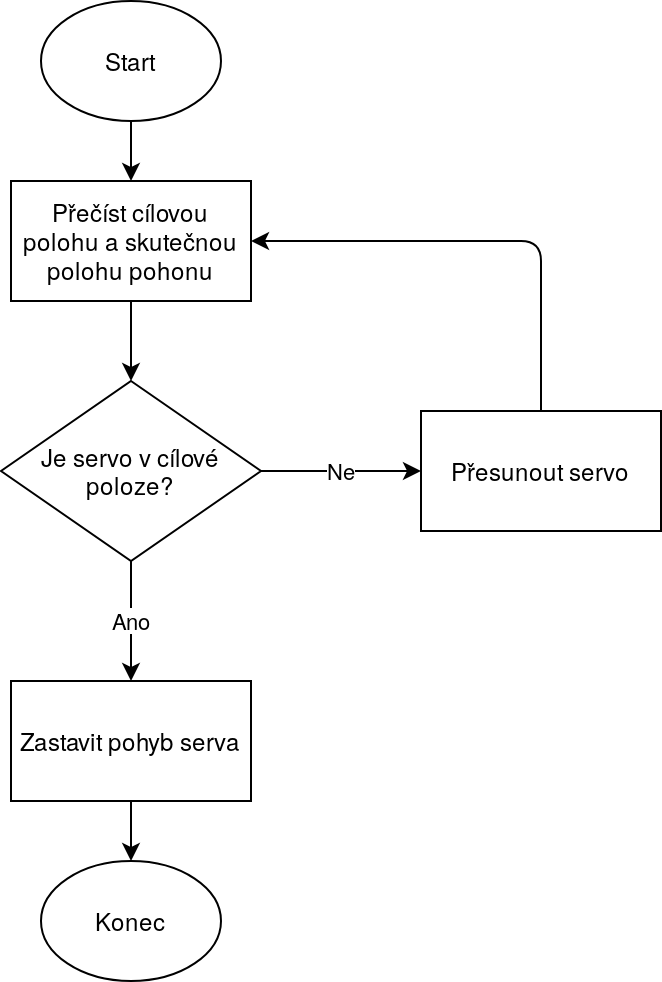
\includegraphics[scale=0.35]{./image/servoAlg.png}
\caption{Řízení modelu}
\label{fig:servoAlg}
\end{figure}


Možným řešením je časové sledování stavu všech servomotorů v ruce. Myšlenka této metody je sledovat polohu každého servomotoru v procesu zavírání nebo otevírání ruky, poté aplikace na základě naměřených výsledků rozhodne, zda zastaví servomotory. Zpočátku víme, původní polohu všech prstů, když je ruka volně otevřena a zavřena (bez předmětu). Vložíme-li objekt do ruky a začneme uzavírat mužeme sledovat změnu v poloze motoru, pak ve chvíli, kdy ruka zasáhne objekt poloha se přestane měnit. Program bude zpracovávat změny a zastaví proces uzavírání ruky. Výhodou tohoto řešení je jednoduchá hardwarová realizace v rámci tohoto projektu, absence potřebnosti přidávání dalších čidel do projektu a minimální změny v původním modelu. Nevýhody jsou nízká přesnost ovládání, nemůžeme udržet moc jemný předmět. 


Základem navrhovaného algoritmu je metoda zpětné vazebné smyčky. Navržené řešení je znázorněno na Obrázku \ref{fig:closeLoop}. Kombinace těchto řešení umožňuje upravit polohu všech prstů pro různé typy úchopů a regulovat zavírání ruky, aby se objekt zachytil.

\begin{figure}[H]
\centering
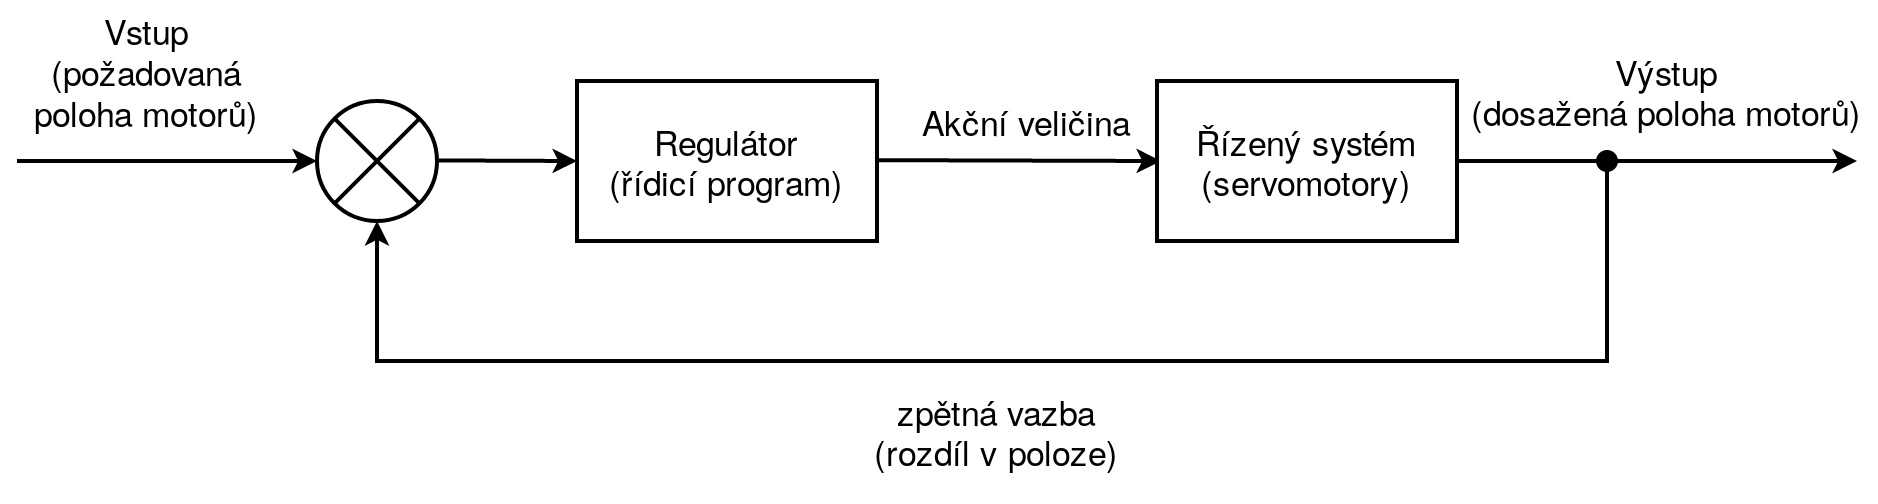
\includegraphics[scale=0.19]{./image/close_loop.png}
\caption{Regulace modelu}
\label{fig:closeLoop}

\end{figure}

\section{Připojení modelu a PC}

Dalším problémem je spojení mezi PC a robotickou rukou. Pro vytvoření aplikace na PC je nutné v modelu implementovat přenos dat do Arduina. Zvoleným řešením je sériová komunikace pomocí kabelu USB.


Všechny desky Arduino obsahují alespoň jeden sériový port (UART nebo USART) určený pro komunikaci s PC nebo jiným zařízením. Arduino navíc obsahuje řadu předem implementovaných funkcí pro čtení (\texttt{Serial.print()}) a zápis (\texttt{Serial.read()}) přes sériový port. Tyto funkce budou použity v programu Arduino Micro, který získá polohu robotické ruky z aplikace na PC a provede model o požadovaného stavu. V PC aplikaci pro ovládání modelu použijeme knihovnu \texttt{termios.h}\cite{termLib}, pomocí které určíme vstupní/výstupní rozhraní pro komunikaci s Arduino Micro.


\section{Ovládání modelu pomocí senzoru}

V původním projektu byl použit svalový senzor ke snímání pohybu paže uživatele. Nevýhodou tohoto řešení je, že pomocí svalových senzorů není možné zjistit přesnou polohu paže. Proto k řešení problému \quoting{ovládání robotické ruky pohybem lidské paže} je vybrán senzor ohybu. 

Senzor ohybu nebo ohybový senzor je senzor, který měří velikost průhybu nebo ohybu. Princip činnosti těchto senzorů je polymerní inkoust, který se nanáší na jednu stranu senzoru. Tento inkoust obsahuje vodivé částice. Když se snímač ohýbá vodivé částice se pohybují dále od sebe a zvyšují odpor\cite{flexSens}. 

Obvykle je senzor přilepen k povrchu a odpor snímacího prvku se mění ohýbáním povrchu. Jako povrch pro tento snímač bude použit prst uživatele, tím pádem výstupní hodnota senzorů bude reprezentovat polohu prstů uživatele. Na základě této hodnoty aplikace bude řídit servomotory, aby robotická ruka dosáhla stejné pozice jako ruka uživatele. 


Navrhovaným řešením pro ovládání modelu pomocí senzoru je ovladač ve tvaru rukavice. Senzory ohybu budou nalepeny na každý prst rukavice. Řídicí jednotkou ovladače bude deska DM Pro Mini Strong. K této desce bude připojeno pět snímačů ohybu. Řídicí jednotka předá hodnoty senzoru do robotické ruky přes PC. Obrázek \ref{fig:gloveBlock} ukazuje blokové schéma celého návrhu projektu.

 \begin{figure}[H]
\centering
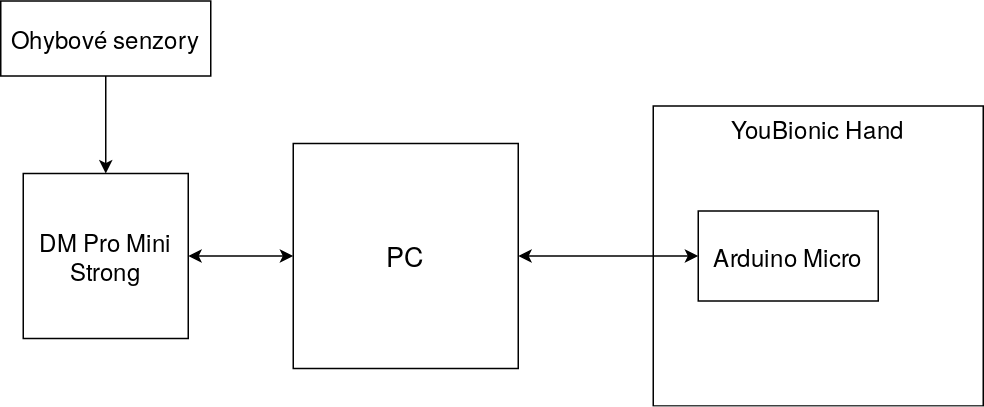
\includegraphics[scale=0.35]{./image/gloveBlock.png}
\caption{Navrhované schéma modelu}
\label{fig:gloveBlock}
\end{figure}

\section{Aplikace}

Demo aplikace by měla ukázat možnosti celého modelu. Kromě toho aplikace spojí řídicí rukavici s robotickou rukou. Pomocí aplikace bude uživatel moci připojit komponenty v rozhraní aplikace, ovládat modelem robotické ruky a sledovat aktuální polohu všech prstů. 


Aplikace by měla obsahovat dvě základní obrazovky. První pro ruční ovládání robotické ruky. Uživatel zadá polohu všech prstů. Poté aplikace odešle tyto polohy do ovladače robotické ruky, který převede model do požadované polohy. Obrázek \ref{fig:wirwframe1} ukazuje wireframe první obrazovky.

 \begin{figure}[H]
\centering
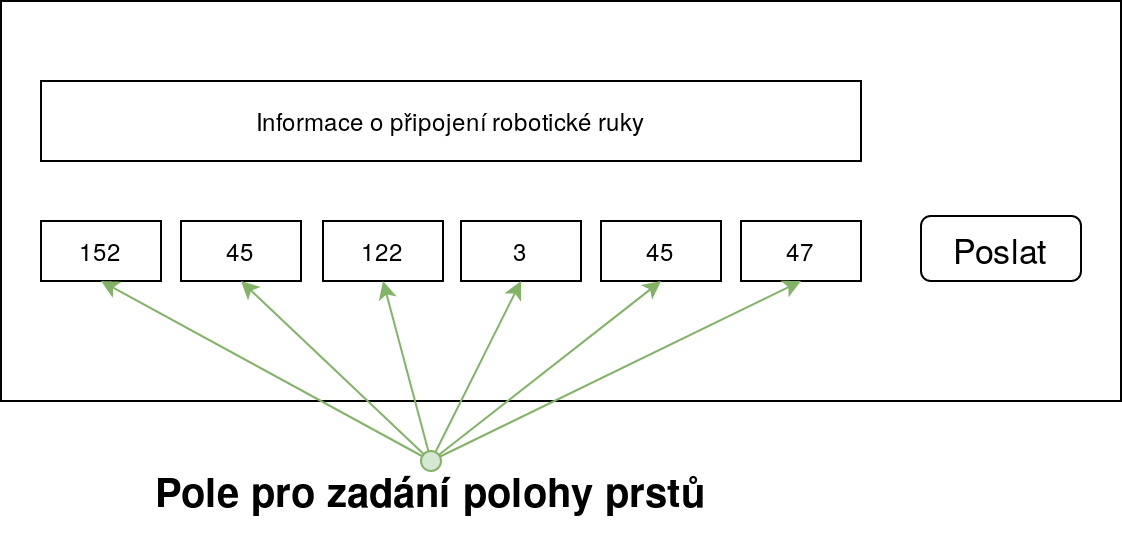
\includegraphics[scale=0.28]{./image/wirwframe1.png}
\caption{První obrazovka aplikace}
\label{fig:wirwframe1}
\end{figure}


Druhá obrazovka je určena k ovládání modelu pomocí rukavice. Uživatel připojí řídicí rukavice k počítači a stiskne tlačítko pro přenos dat z rukavice do robotické ruky.


Pro snadnější implementaci aplikace a vývoj projektu v budoucnu je nutné napsat knihovnu pro ovládání modelu. Tato knihovna umožní práci s modelem v dalších projektech a umožní rozšíření existujících řešení.  


K implementaci aplikace byla vybrán framework \texttt{GTK}. Je to otevřený nástroj pro vytváření grafických uživatelských rozhraní. Zvolený programovací jazyk pro vytvoření aplikace je C.


K implementaci grafického rozhraní bude použit program \texttt{Glade}\cite{gladePr}. To je aplikace pro vytváření grafického rozhraní na zakladě knihovny \texttt{GTK}. 


\chapter{Realizace}

Tato kapitola popisuje implementaci řešení navržených v předchozí kapitole. Podrobně vysvětleny hardwarové změny v modelu pro jednodušší rozšíření projektu do budoucnosti. Představena aplikace pro demonstraci možnosti modelu. Jsou popsány implementované programy pro komponenty projektu.

\section{Připojení a komunikace mezi komponenty}

Pro přístup k potenciometrům v servomotorech byla původní deska přepájena a zpětná vazba servomotoru byla vyvedena na externí port (Obrazek \ref{fig:PortFeedback}). K tomuto portu je připojena deska DM Pro Mini Strong pomocí drátů. Tabulka \ref{tab:FeedbackPort} ukazuje implementované připojení potenciometrů servomotorů k řídicí desce.

\hspace{3cm}

\begin{minipage}{\textwidth}
  \begin{minipage}[b]{0.29\textwidth}
    \centering
    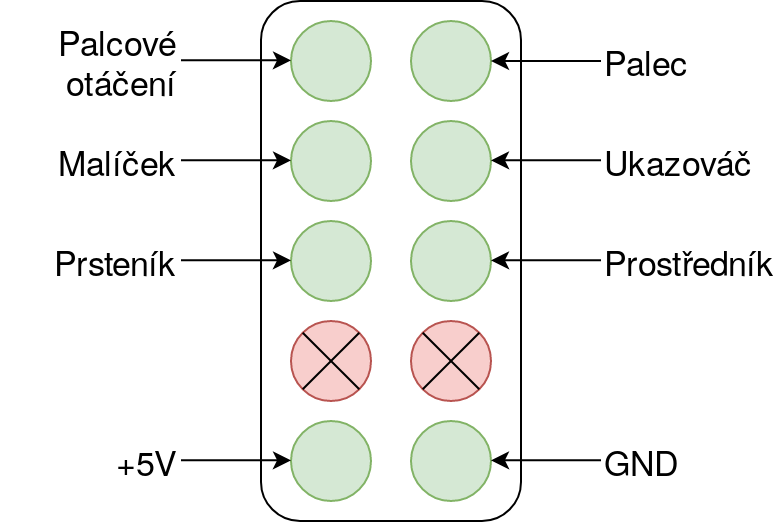
\includegraphics[scale=0.2]{./image/PortFeedback.png}
    \captionof{figure}{Port potenciometrů}
    \label{fig:PortFeedback}
  \end{minipage}
  \hfill
  \begin{minipage}[b]{0.8\textwidth}
    \centering
\begin{tabular}{|l|l|}
\hline
\textbf{Potenciometr} & \textbf{Pin} \\ \hline
Ukazováč        & A0  \\ \hline
Prostředník     & A1  \\ \hline
Prsteník        & A2  \\ \hline
Malíček         & A3  \\ \hline
Palec           & A4  \\ \hline
Palcové otáčení & A5  \\ \hline
\end{tabular}
      \captionof{table}{Připojení potenciometrů}
      \label{tab:FeedbackPort}
    \end{minipage}
  \end{minipage}

\hspace{3cm}

Komunikace mezi ovladačem robotické ruky a externí deskou realizovaná prostřednictvím knihovny \texttt{SPI.h}. Funkce \texttt{SPIgetServoPositions()} byla implementována na straně Master, která používá funkci \texttt{transferAndWait()} k dodání hodnoty potenciometru zpětné vazby servomotoru z externí desky. Pomocí funkce \texttt{SPI.transfer()} Master vysila číslo požadovaného potenciometru a vyvolá přerušení na straně slave. Implementováa obsluha přerušení, ve které Slave na základě přijatých dat předava hodnoty vstupních signálů z potenciometrů servomotorů. Tabulka \ref{tab:MastSlaveKom} ukazuje vztah mezi přijatou a odeslanou hodnotou na zařízení Slave.

 \begin{table}[h]
 \centering
\begin{tabular}{|l|l|}
\hline
\textbf{Přijatá hodnota} & \textbf{Odeslaná hodnota} \\ \hline
1                         & hodnota na A0              \\ \hline
2                         & hodnota na A1              \\ \hline
3                         & hodnota na A2              \\ \hline
4                         & hodnota na A3              \\ \hline
5                         & hodnota na A4              \\ \hline
6                         & hodnota na A5              \\ \hline
\end{tabular}
\captionof{table}{Slave odesílání}
\label{tab:MastSlaveKom}
\end{table}


Řídicí jednotka robotické ruky čte požadovanou polohu ze sériového portu. Pak přivádí model do požadovaného stavu. Obrázek \ref{fig:CommFormat} ukazuje implementovaný formát, ve kterém ovladač robotické ruky přijímá informace o požadované poloze. Po zastavení všech servomotorů pošle řídicí jednotka aktuální polohy pohonů. Stejný formát byl použit pro příjem a odeslání pozice motoru.


 \begin{figure}[h]
\centering
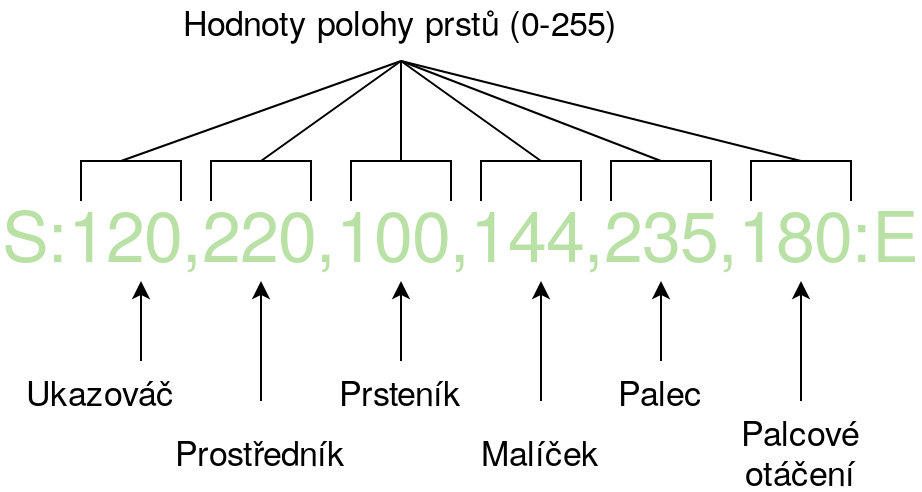
\includegraphics[scale=0.31]{./image/CommFormat.png}
\caption{Formát příkazu}
\label{fig:CommFormat}
\end{figure}

Pro ilustraci změn provedených v modelu a pro demonstraci propojení všech komponent, bylo vytvořeno schéma připojení komponentů v projektu. Schéma znázorněné na Obrázku \ref{fig:HandScheme} a přidané k elektrickým přílohám díla.


 \begin{figure}[H]
\centering
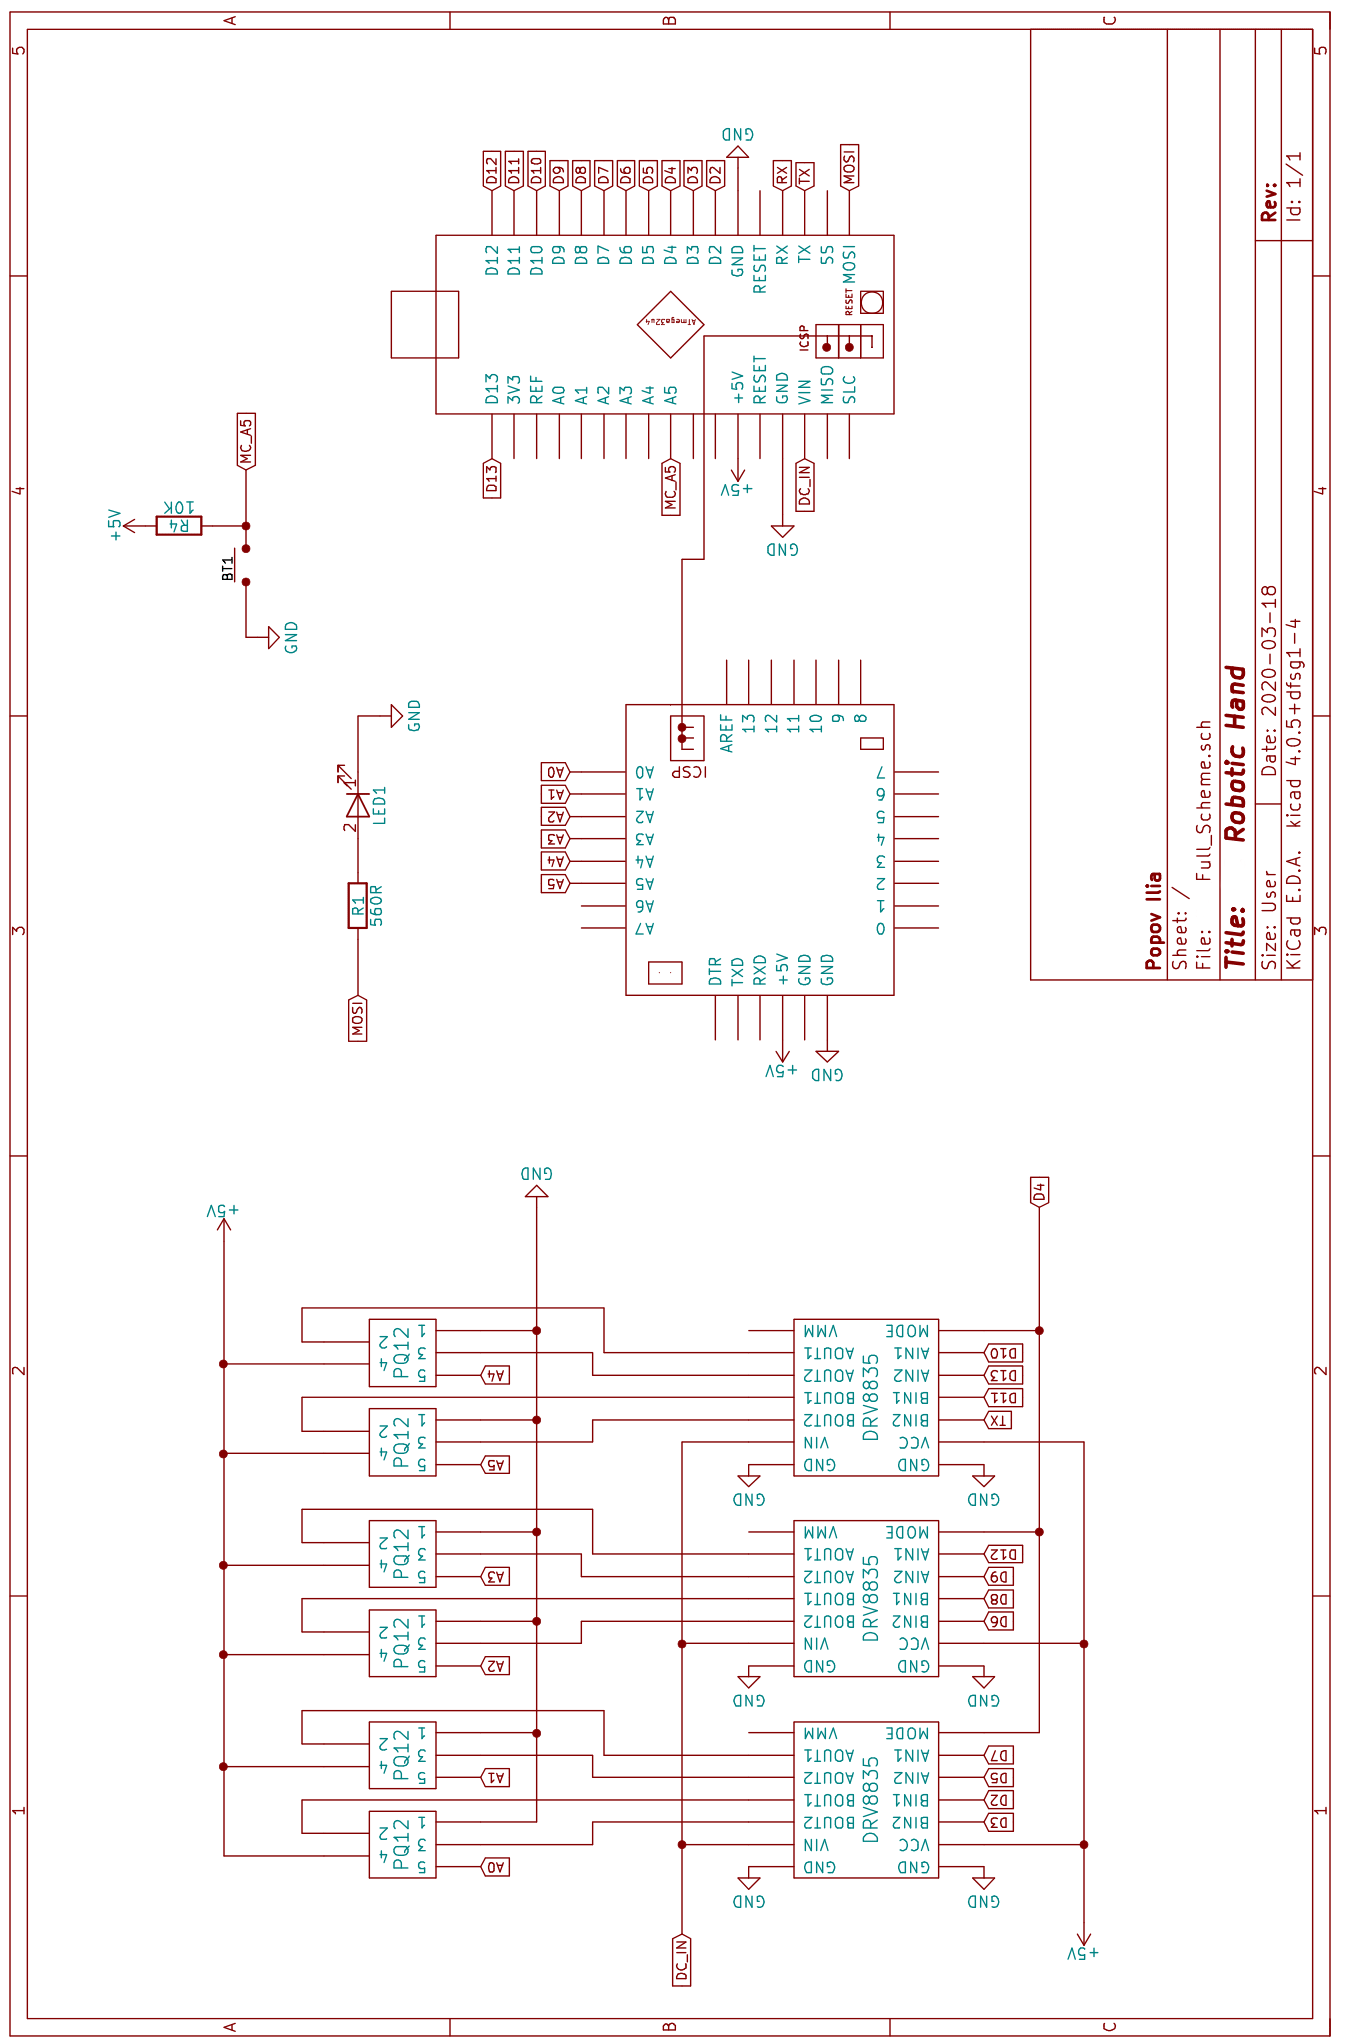
\includegraphics[scale=0.27]{./image/HandScheme.png}
\caption{Schéma zapojení komponentů}
\label{fig:HandScheme}
\end{figure} 


Po provedení všech změn v návrhu byl model znovu sestaven. Konečný výsledek je znázorněn na Obrázku \ref{fig:finalHand}.

 \begin{figure}[h]
\centering
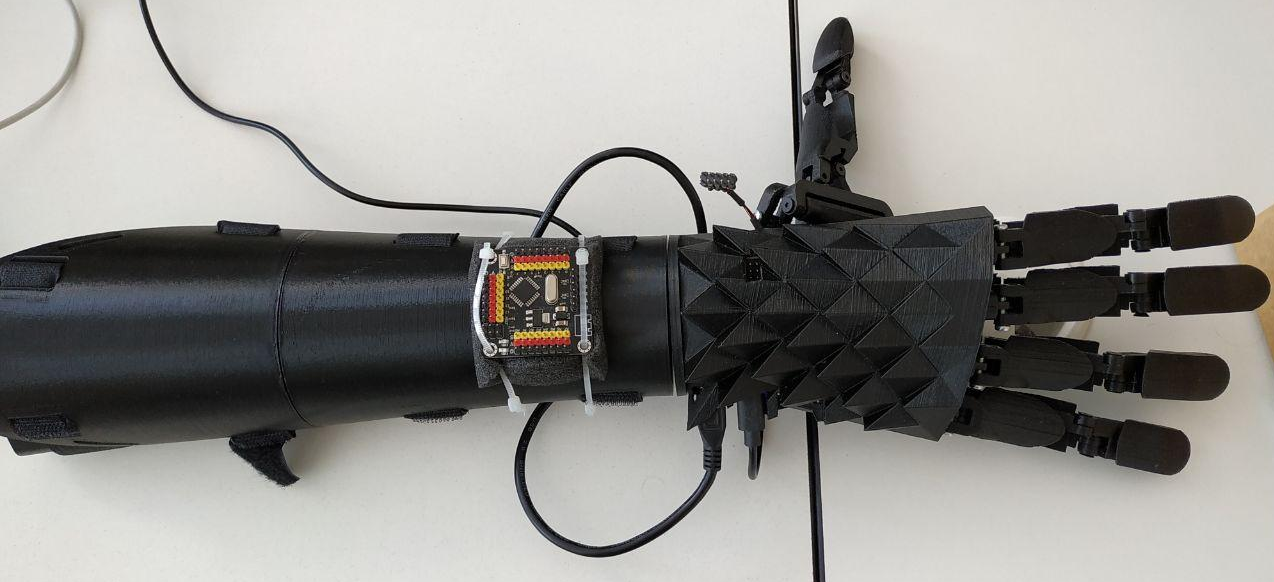
\includegraphics[scale=0.35]{./image/handFinal.png}
\caption{Sestavený model ruky}
\label{fig:finalHand}
\end{figure} 

\section{Rukavice}

V rámci této práce byl navržen a implementován řadič, ve tvaru rukavice(\ref{fig:gloveFoto}), pro ovládání robotické ruky ohýbáním paže uživatele. Senzory ohybu byly přilepeny na každý prst pracovní rukavice.

 \begin{figure}[h]
\centering
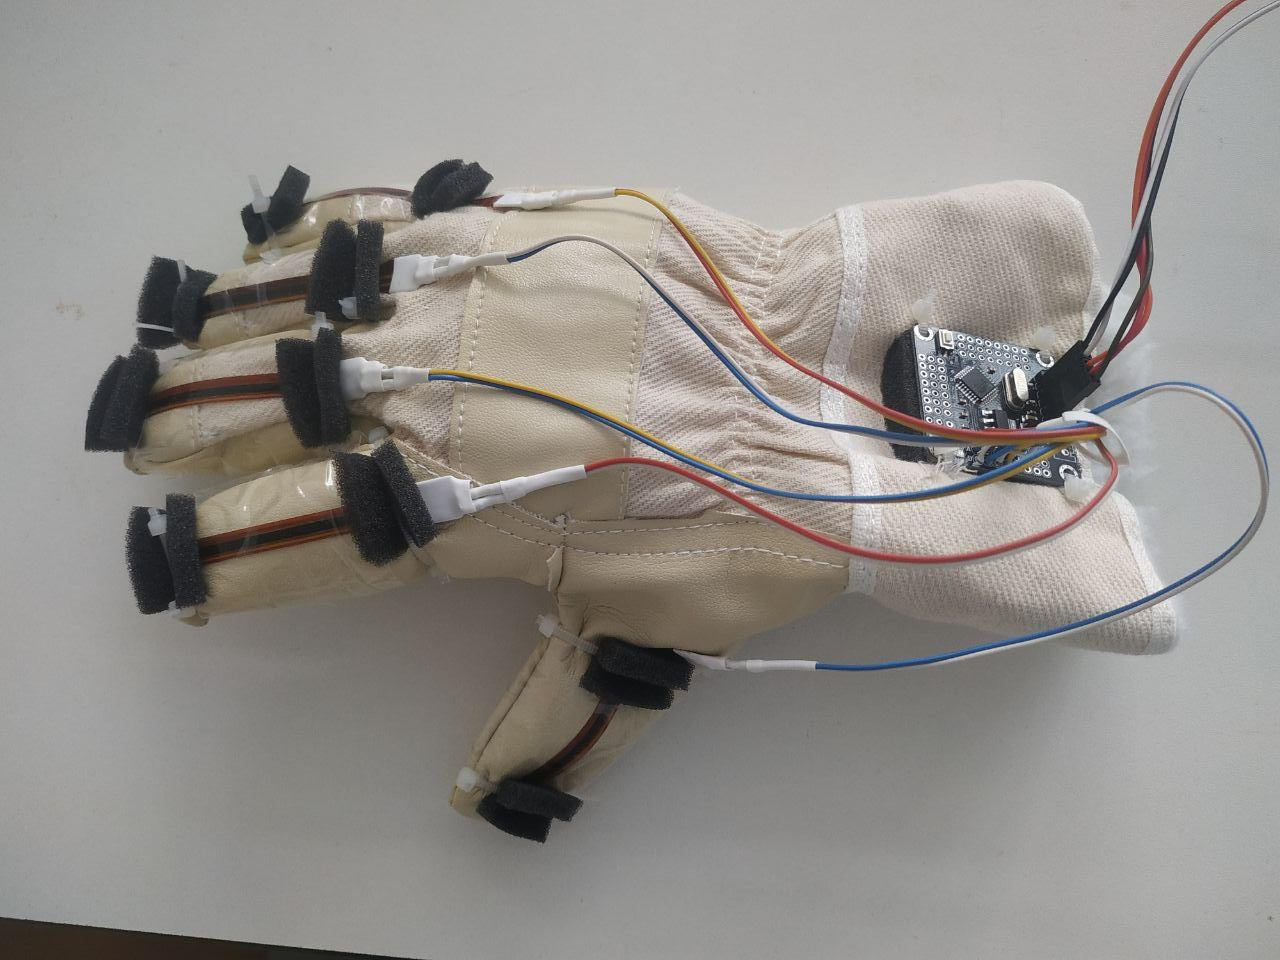
\includegraphics[scale=0.33]{./image/glove.jpg}
\caption{Rukavice}
\label{fig:gloveFoto}
\end{figure} 

Senzory jsou propojeny do ovládací desky přes odpor způsobem znázorněným na Obrázku \ref{fig:flexSensConn}. 

 \begin{figure}[h]
\centering
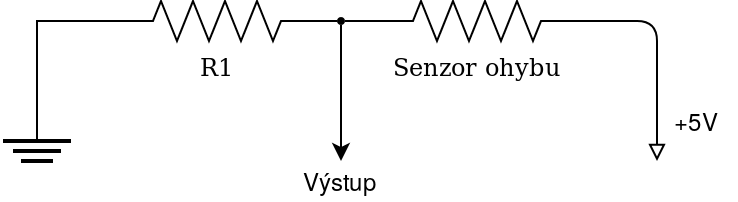
\includegraphics[scale=0.37]{./image/flexSensConn.png}
\caption{Připojení senzoru ohybu}
\label{fig:flexSensConn}
\end{figure} 

Optimální hodnota odporu se rovná 47KOm a byla spočítána z výrazu pro výstupní napětí této schématy: $V_{out} = \frac{V^+}{1 + \frac{R_1}{R_2}}$. Tato hodnota má největší rozsah výstupní hodnoty při ohýbání senzoru. Uvedený odpor byl použit při implementaci.


V této práci byly použity oboustranné ohybové senzory (senzor se ohýbal ve dvou směrech). Model ruky a lidská paže se ohýbají pouze v jednom směru, proto k ovladači byla připojena pouze jedna strana každého senzoru. 

Realizované schéma zapojení je znázorněno na Obrázku \ref{fig:SchGlove}. Řídicí jednotka zpracovává hodnoty senzorů a odesílá ve formátu používaném v ovladači robotické ruky k získání požadované polohy prstů modelu. Tabulka \ref{tab:gloveConn} ukazuje připojení prstů rukavice ke vstupním signálům řídicí jednotky.


\begin{table}[H]
\centering
\begin{tabular}{|l|l|}
\hline
\textbf{Prst na rukavici} & \textbf{PIN} \\ \hline
Ukazováč                  & A0           \\ \hline
Prostředník               & A1           \\ \hline
Prsteník                  & A2           \\ \hline
Malíček                   & A3           \\ \hline
Palec                     & A4           \\ \hline
\end{tabular}
\caption{Připojení prstů rukavice}
\label{tab:gloveConn}
\end{table}



 \begin{figure}[H]
\centering
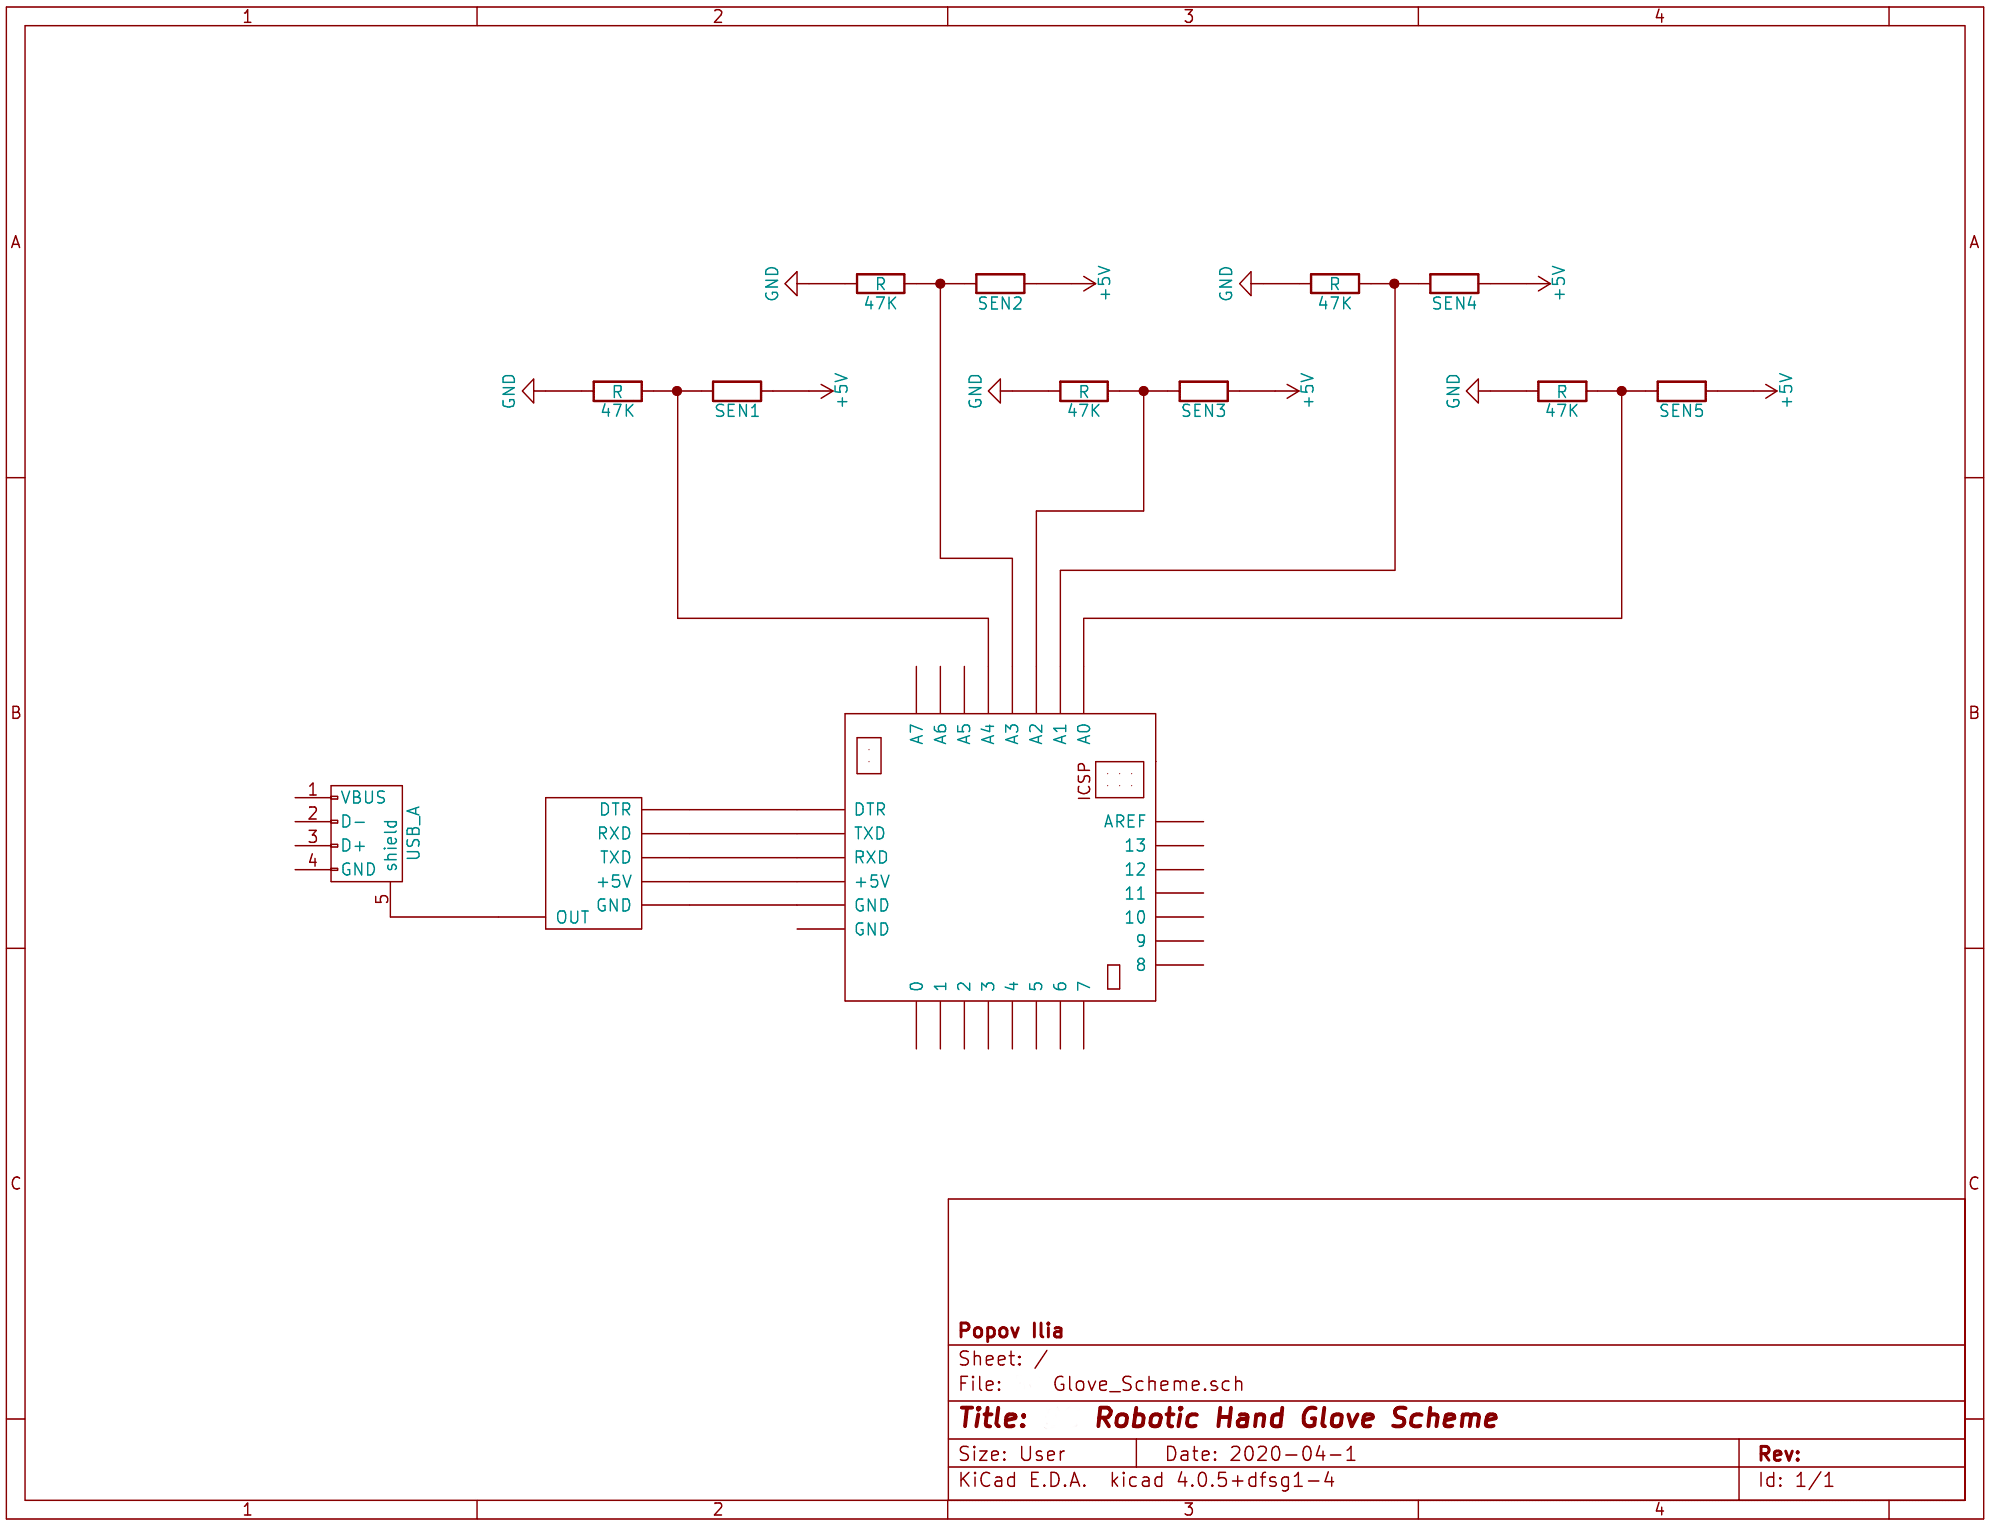
\includegraphics[scale=0.185]{./image/SchGlove.png}
\caption{Schéma zapojení rukavice}
\label{fig:SchGlove}
\end{figure} 


  
 
\section{Řídicí programy}

Tato podkapitola popisuje implementované skripty pro všechny řídicí jednotky používané v práci. Všechny kódy popsané v této kapitole jsou součástí elektronické verze této práce a jsou popsány pomocí komentářů. 

Všechny komponenty použité v projektu jsou desky Arduino nebo s nimi kompatibilní. Programy pro Arduino obsahují dvě základní funkce \texttt{setup()} a \texttt{loop()}. První se volá po zapnutí desky a používá se k inicializaci. Druhá funkce je určena pro hlavní část kódu a je volána cyklicky po celou dobu napájení desky.

\subsection{Řídicí deska v robotické ruce}

Program implementovaný pro hlavní řídicí jednotku robotické ruky, přijímá požadovanou polohu prstu robotické ruky přes sériový port ve formátu popsaném v předchozí podkapitole(Obrázek \ref{fig:CommFormat}). 

Program pak kontroluje správnost přijatých dat. Poloha každého prstu má rozsah pro nastavení 0-255, kde 0 - prst je zavřený a 255 - maximální otevřený. Při zadávání záporné hodnoty do polohy libovolného prstu program ponechá vybraný prst v původní poloze. Model nebude reagovat na jiné změny formátu nebo nesprávný vstup. 

Po přijetí platné zprávy pro nastavení modelu program sleduje aktuální polohu pohonu a porovná ji s požadovanou pozicí. Na základě tohoto srovnání ovladač pohybuje servopohony a pak znovu porovnává polohy. 

Proces porovnávání polohy a pohybu servopohonu se provádí, dokud pohon nedosáhne požadované polohy nebo nepřestane měnit svou polohu (v případě selhání pohonu, došlo k výpadku napájení pohonu, překážce v pohybu). 

Po zastavení všech servomotorů se program vrátí do původního stavu, kde čeká na další vstup. Obrázek \ref{fig:ArdMProgDiagram} odkaz ukazuje vývojový diagram implementovaného programu. 

Pro jednoduchost použití a přehlednost v kódu aplikace byla realizována struktura \texttt{SFinger} \ref{code:structTFing}, která reprezentuje prst modelu robotické ruky v kódu aplikace. V každé instance této třídy jsou uloženy výstupní piny pro řízení servomotorů, číslo prstu, pozice, která má být dosažena a pro přesnost ovládání jsou uloženy dvě poslední změřené pozice servomotorů. 



\begin{lstlisting}[caption={Reprezentace motoru},label={code:structTFing}]

struct SFinger {
  int pinDir;
  int pinPwm;
  int fingerPos;
  int fingerPrevPos;   
  int fingerID;
  int targetPos;
  };
  
\end{lstlisting}

\newpage

 \begin{figure}[H]
\centering
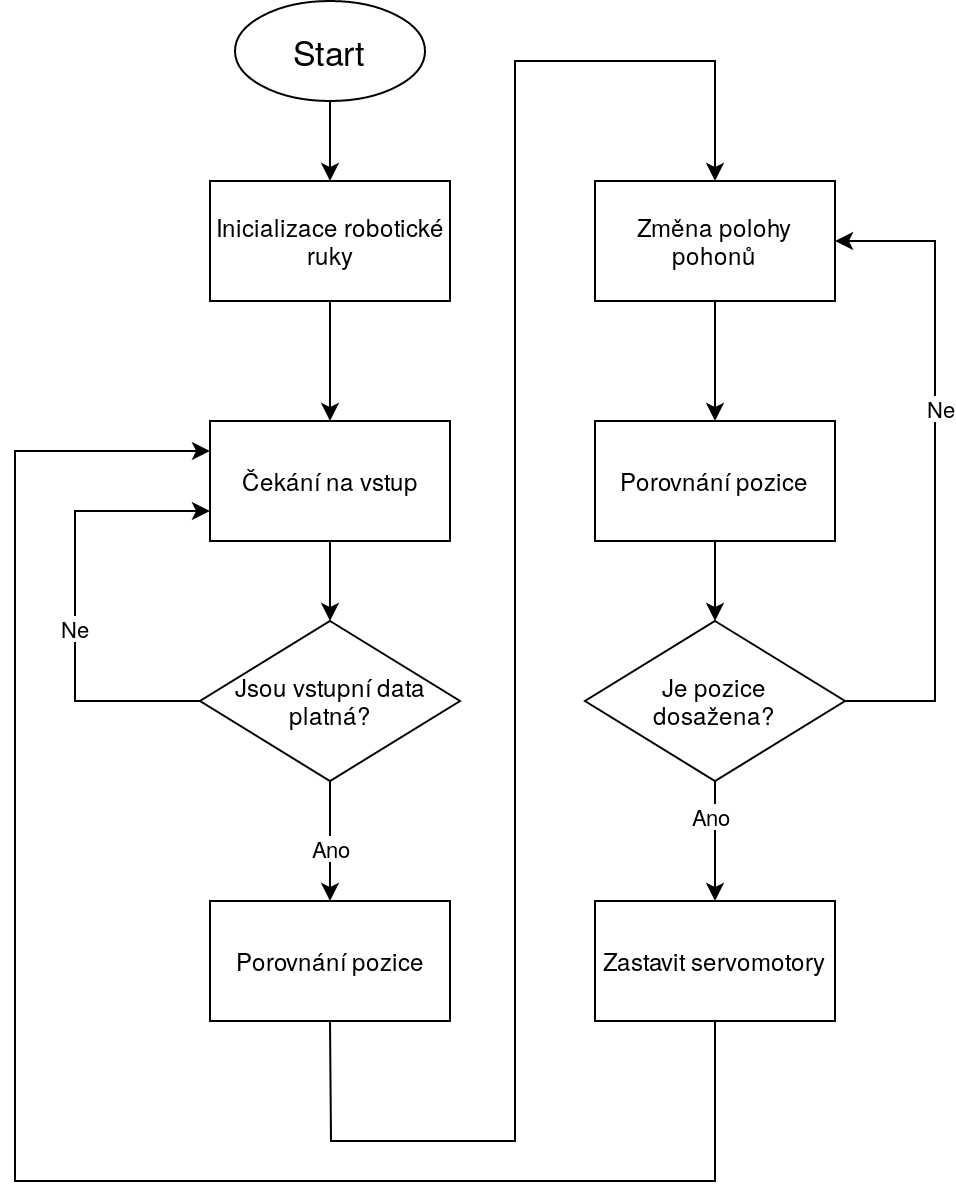
\includegraphics[scale=0.3]{./image/ArdMProgDiagram.png}
\caption{Program pro hlavní řídicí jednotku robotické ruky}
\label{fig:ArdMProgDiagram}
\end{figure} 



\subsection{Externí deska v robotické ruce}

Program pro externí desku, ke které jsou připojeny zpětné vazby servopohonů, nepřetržitě čte a ukládá aktuální hodnoty potenciometrů. 

Při volání přerušení ze zařízení Master, řídicí jednotka odešle jednu z uložených hodnot polohy pohonu. Funkce \texttt{SPI.transfer()} z knihovny \texttt{SPI.h}, použitá na straně Master pro předávání dat, podporuje velikost dat 8 bitů. Proto jsou naměřené a následně odeslané hodnoty přiřazeny k rozsahu 0-255. Obrázek \ref{fig:ExtDeskProgDiag} ukazuje vývojový diagram implementovaného programu.

\newpage

 \begin{figure}[H]
\centering
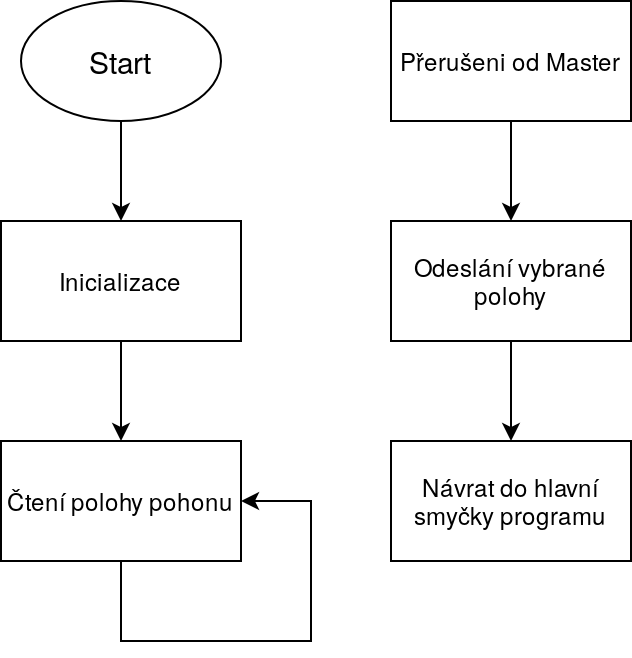
\includegraphics[scale=0.35]{./image/ExtDeskProgDiag.png}
\caption{Formát příkazu}
\label{fig:ExtDeskProgDiag}
\end{figure} 

\subsection{Řídicí jednotka rukavice}

Implementace řídicí jednotky ovladače je podobná programu pro externí desku v robotické ruce. Hlavním rozdílem je způsob komunikace. Ovladač komunikuje přes sériový port. 

Program čeká na požadavek na sériovém portu. Po přijetí zprávy ovladač pošle polohu všech prstů do srukavice ve formátu pro řídicí jednotku robotické ruky (Obrázek \ref{fig:CommFormat}). 


Protože robotické rameno nastavuje šest motorů, má-li rukavice pouze pět senzorů pro sledování polohy prstu uživatele, byla k odeslané hodnotě přidána hodnota -1 pro polohu otáčení palce. To umožňuje přenos dat přímo z rukavice do řídicí jednotky bez jakýchkoli změn za předpokladu, že poloha otáčení palce zůstává nezměněna. 

Obrázek \ref{fig:GloveProgDiagr} ukazuje vývojový diagram implementovaného programu.

\newpage

 \begin{figure}[H]
\centering
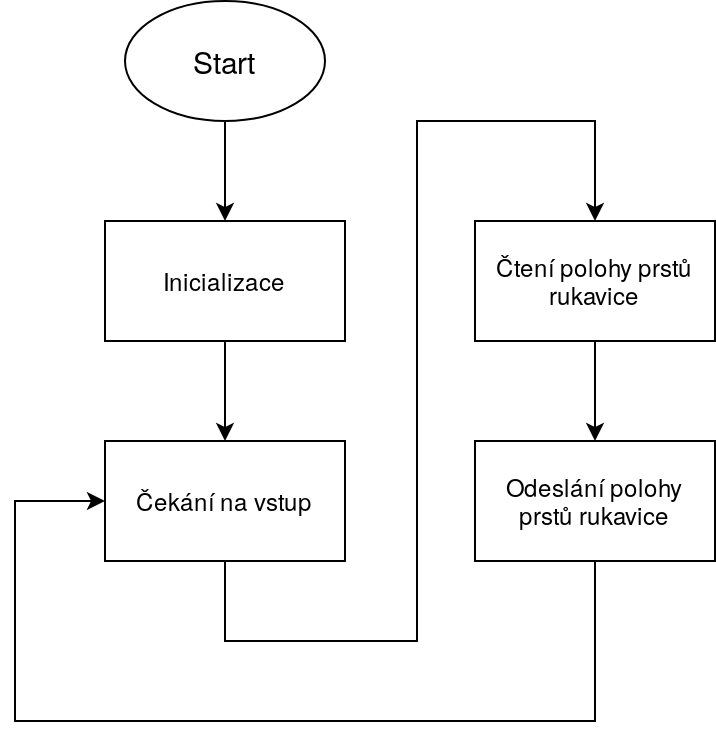
\includegraphics[scale=0.35]{./image/GloveProgDiagr.png}
\caption{Formát příkazu}
\label{fig:GloveProgDiagr}
\end{figure} 



\section{Knihovna}

Pro ovládání modelu v navržené demo aplikaci nebo v jiném PC programu, byla vytvořena knihovna \texttt{Hand.h} v jazyce C. 

Knihovna obsahuje funkci pro připojení k modelu robotické ruky a dalším zařízením použítým v této práci přes sériový port. Takže knihovna obsahuje funkci ovládání modelu a přeposílání dat mezi zařízeními. Pro reprezentaci zařízení byla vytvořena struktura \texttt{SArdDev}. Ve struktuře jsou uloženy adresa zařízení a stav připojeni. Knihovna také obsahuje strukturu \texttt{SSerial}, ve které jsou uložena nastavení pro komunikaci se zařízením a původní nastaveni.


Popis základních funkcí knihovny uveden v Tabulce \ref{tab:lib}. Podrobný popis struktur a funkci knihovny jsou uvedeny v přílohách.

\newpage

\begin{table}[H]
\begin{tabular}{|l|l|}
\hline
\textbf{Funkce}                                                                                  & \textbf{Popis}                                                                                                                                                                                                \\ \hline
\begin{tabular}[c]{@{}l@{}}openDevice \\ (SArdDev* device, const char* addr)\end{tabular}        & \begin{tabular}[c]{@{}l@{}}Funkce inicializuje \\ zařízení na adrese addr.\\ Struktura SArdDev představuje \\ zařízení v knihovně.\\ Vrací true při úspěšné \\ inicializaci a false při selhání.\end{tabular} \\ \hline
\begin{tabular}[c]{@{}l@{}}readFromArd \\ (SArdDev device, char* buff, int size)\end{tabular}    & \begin{tabular}[c]{@{}l@{}}Funkce čte data ze zařízení \\ device do pole buff.\end{tabular}                                                                                                                   \\ \hline
\begin{tabular}[c]{@{}l@{}}openHand \\ (SArdDev* device)\end{tabular}                            & \begin{tabular}[c]{@{}l@{}}Funkce odešle příkaz otevření \\ robotické ruky do zařízení device.\end{tabular}                                                                                                   \\ \hline
\begin{tabular}[c]{@{}l@{}}closeHand \\ (SArdDev* device)\end{tabular}                           & \begin{tabular}[c]{@{}l@{}}Funkce odešle příkaz uzavření \\ robotické ruky do zařízení device.\end{tabular}                                                                                                   \\ \hline
\begin{tabular}[c]{@{}l@{}}sendStatesToHand \\ (SArdDev* device, int states{[}6{]})\end{tabular} & \begin{tabular}[c]{@{}l@{}}Funkce odešle příkaz \\ k nastavení všech prstů \\ robotické ruky na pozice\\ uložené v poli states\end{tabular}                                                                   \\ \hline
\end{tabular}
\caption{Zakladní funkci knihovny}
\label{tab:lib}
\end{table}

\section{Aplikace}

Na základě implementované knihovny pro řízení modelu a knihovny \texttt{GTK} pro implementace uživatelského rozhraní byla vytvořena aplikace pro demonstraci funkcí modelu robotické ruky. GUI aplikace vytvořené v aplikaci Glade. Popis vytvořeného rozhraní uložen v XML souborech. Vytvorena aplikace připojuje rozhraní pomocí objektu \texttt{GtkBuilder}. 


Aplikace má tři základní obrazovky pro různé způsoby ovládání modelu a obrazovku Menu pro přepínání mezi obrazovkami. Pro komunikaci mezi obrazovkami, objekty aplikace a sledování stavu aplikace byla implementována struktura \texttt{app\_widgets}, která je přístupná z funkcí všech objektů aplikace. Tato struktura obsahuje odkazy na všechny objekty používané v aplikaci, uložené struktury pro připojení komponent modelu a stav aplikace a připojenych komponentů. Po spuštění aplikace inicializuje všechny obrazovky, objekty GUI a konfiguruje komunikační parametry. 


Všechny obrazovky obsahují pole pro zadání adresy zařízení a tlačítko připojení. Jakmile je model robotické ruky připojen, informace o stavu připojení a poloha prstů modelu budou viditelné na všech obrazovkách aplikace. Při zavření jakékoli obrazovky, program zničí všechny objekty, vrátí parametry změněné v aplikaci na výchozí nastavení a ukončí aplikaci.

\newpage

\subsection{Obrazovka ovládání přes rukavice}

První obrazovka je určena k ovládání modelu pomocí rukavice. Uživatel zde může připojit model robotické ruky a ovladač rukavice. Po připojení robotická ruka bude kopírovat aktuální polohu rukavice. 


Implementovaný model ovladače ve tvaru rukavice zachycuje polohu všech prstů. Robotický model kromě nastavení polohy všech prstů  má možmost nastavit polohu otáčení palce. Proto byla v aplikaci implementována funkce ručního zadávání polohy otáčení palce. Poloha otáčení palce se zadává do konkrétního pole obrazovky. Tuto funkci lze vypnout zaškrtnutím políčka vedle pole. Když je tato funkce vypnutá, poloha otáčení palce se nezmění.


V aplikace implementovana funkce cteni a zobrazeni polohy prstu ovladaci rukavice. Po stisknutí tlačítka \texttt{Read data from glove} aplikace zkontroluje připojení rukavice. A pak pomocí funkce \texttt{g\_timeout\_add\_full} z knihovny \texttt{GTK} periodicky vyvolává implementovanou funkci čtení dat ze sériového portu, ke kterému je rukavice připojena. Přečtená poloha prstů rukavice se zobrazí na obrazovce.


Po použití tlačítka \texttt{Start}, aplikace zkontrolujte připojení komponentů. Poté bude pravidelně čistit polohy prstů rukavice a předávat je modelu robotcké ruky.


 \begin{figure}[H]
\centering
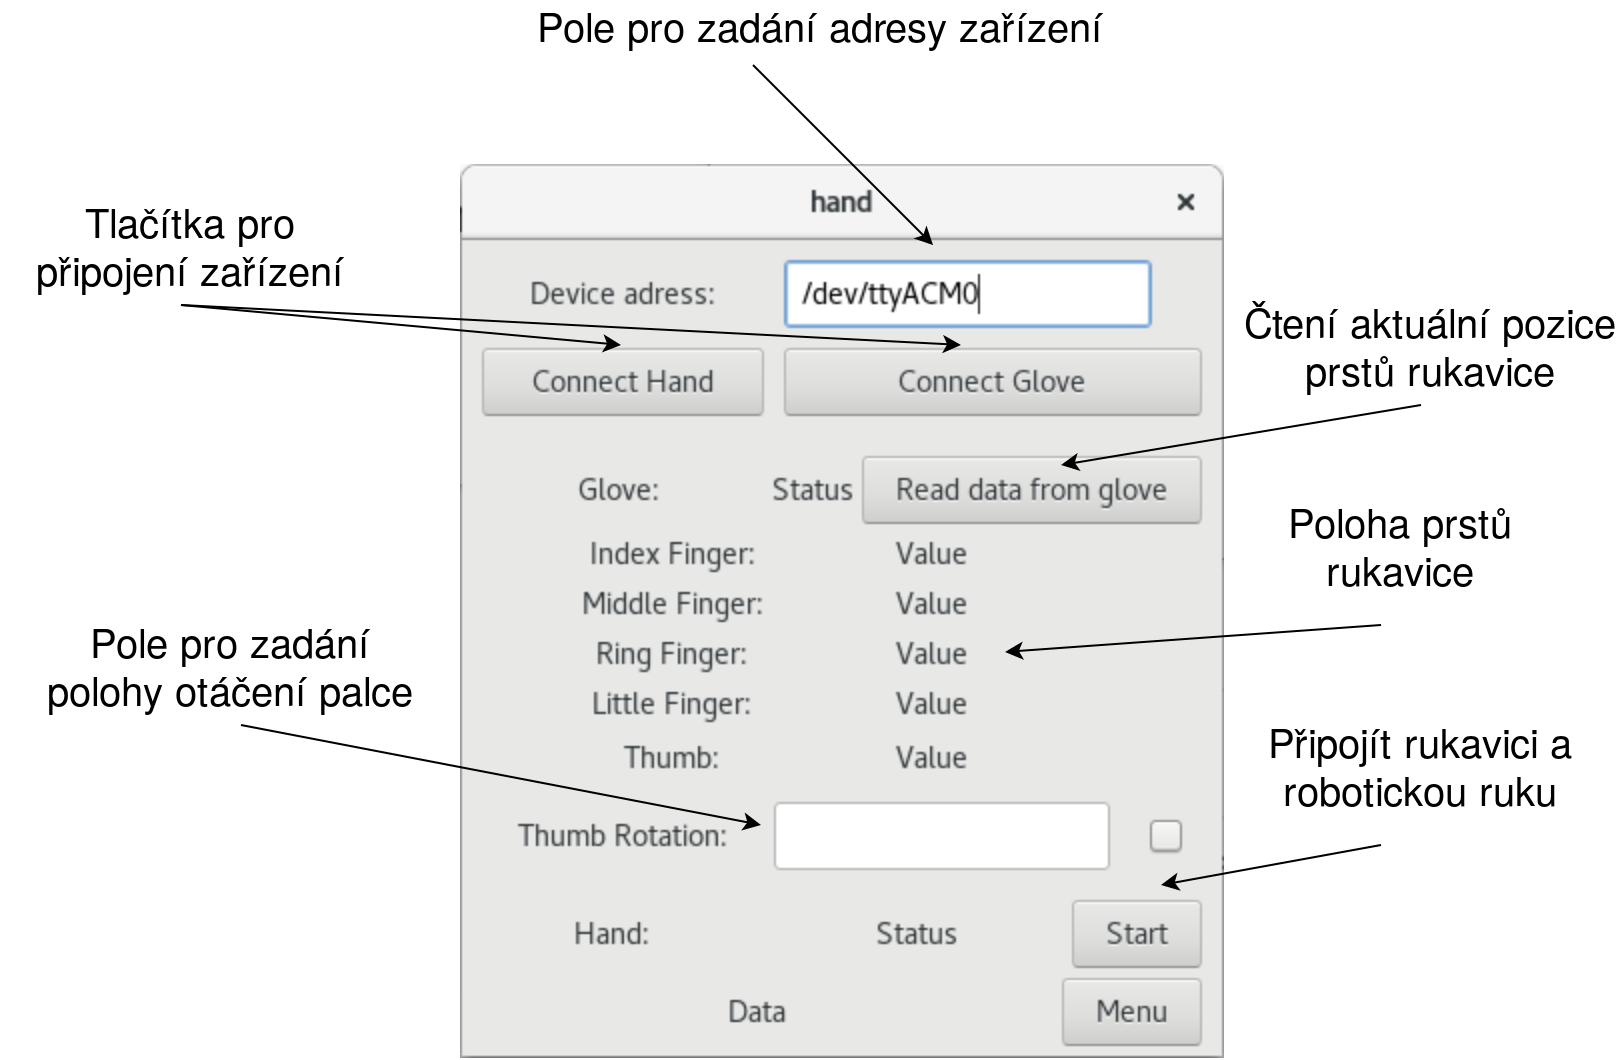
\includegraphics[scale=0.22]{./image/AppScreen1.png}
\caption{Obrazovka ovládání přes rukavice}
\label{fig:AppScreen1}
\end{figure} 


\newpage

\subsection{Obrazovka manuálního ovládání}


Druhá obrazovka je určena k ručnímu nastavení robotické ruky do polohy určené uživatelem. Zde může uživatel nastavit polohu všech prstů robotické ruky zvlášť. Pozice se zadávají do určitých polí na obrazovce. Je implementována funkce změny polohy pouze vybraných prstů. Prsty lze vybrat pomocí zaškrtávacích políček.

Stisknutím tlačítka \texttt{Send to Hand} aplikace kontroluje zadané pozice a přeposílá je do modelu. Pro odeslání byla použita funkce \texttt{sendStatesToHand} z implementované khihiovny. 


 \begin{figure}[H]
\centering
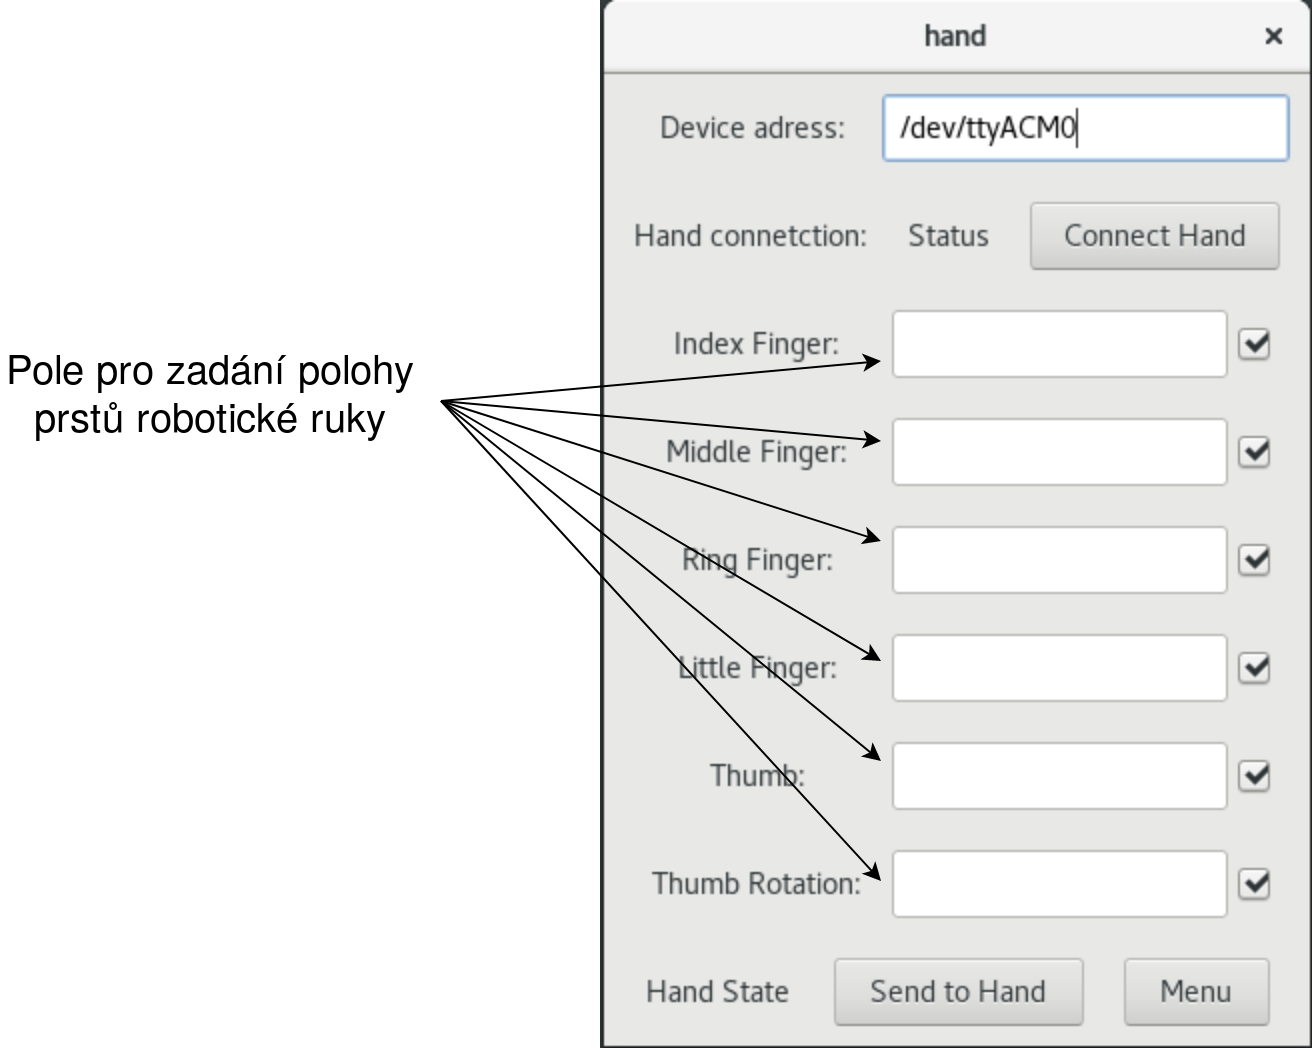
\includegraphics[scale=0.22]{./image/AppScreen2.png}
\caption{Obrazovka manuálního ovládání}
\label{fig:AppScreen2}
\end{figure} 

\newpage

\subsection{Obrazovka přednastavených stavu}

Poslední obrazovka obsahuje několik přednastavených pozic robotické ruky, které demonstrují možnosti modelu. Na této obrazovce jsou implementovány pohyby otevírání a zavírání ruky. Takže jsou implementovány přednastavené polohy pro různé způsoby uchopení předmetů, které byly popsány v kapitole \ref{sec:hand}. S těmito pozicemi se uživatel může pokusit zachytit různé objekty pomocí robotcké ruky. 

Pro otestovani uchopeni, je potřeba model nastavit do jedné z pozic a poté pomocí tlačítka \texttt{Close hand} zavřít robotickou ruku. V aplikaci je implementováno několik gestů, které jsou vhodný pro prezentaci modelu a jeho možnosti.

 \begin{figure}[H]
\centering
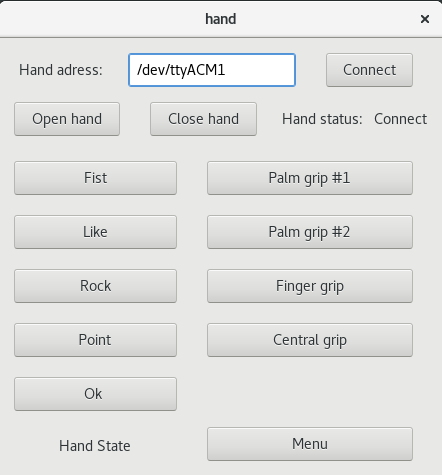
\includegraphics[scale=0.5]{./image/AppScreen3.png}
\caption{Obrazovka přednastavených stavu}
\label{fig:AppScreen3}
\end{figure} 


\chapter{Testování řešení}
\label{ch:testSol}

Na modelu YouBionic Hand byla otestována knihovna pro ovládání robotické ruky a ukázková aplikace pro demonstraci možnosti modelu. Videa ovládání modelem pomocí rukavice a uchopení předmětu robotckou rukou jsou na přiloženém CD. Fotografie z testování modelu lze nalézt v příloze. 


\section{Testování robotické ruky}

Pro testování realizováného řešení pro robotickou ruku byl použit Arduino IDE a implementováný do IDE Sériový monitor. Sériový monitor je nástroj pro komunikaci s připojením Arduino přes sériovou linku.


Testování probihalo na zakladě připojení Arduino v robotické ruce k PC a následním odesláním polohy servomotoru přes Sériový monitor. Pro testování byla vytvořena série testů, ve kterých byla pozorována poloha servomotorů robotické ruky.


Testování bylo provedeno na dvou úrovních. V prvním bylo testováno dosažení modelu požadovaných poloh motoru bez překážek v pohybu. Byla testována změna pozic všech prstů samostatně a současné nastavení pozic všech prstů. Ve všech testech robotická ruka dosáhla požadovaných poloh prstů s odchylkou v poloze motorů 5-8\%.


Druhý test ověřoval schopnost modelu zastavit prsty robotické ruky a chytit předmět. Pro testování byly použity předměty z kapitoly \ref{ch:test}. Ve všech pokusech byl model schopen zastavit servomotory při překážkách v pohybu. Po zastavení motoru je v robotické ruce pevně držen předmět, který je překážkou v pohybu.


Díky implementovanému řešení byla robotická ruka při testování schopna držet tužku způsobem vhodným pro psaní. Video testu lze nalézt v přiloženém CD. Fotografie z testů jsou uvedeny v příloze práce.

\section{Testování aplikací a rukavice}

Před testováním aplikace byla knihovna, implementovaná pro řízení modelu, testována samostatně. Všechny funkce knihovny fungují podle definovaných požadavků. Při komunikaci s modelem prostřednictvím knihovny model reaguje stejně jako při ovládání pomocí Arduino IDE.


Všechny aplikační funkce byly testovány a fungují podle definice. Při propojení ovladače rukavice a modelu robotického ramene aplikace realizuje řízení modelu pohybem uživatele. Zjištěným nedostatkem v řešení je rychlost reakce robotické ruky na změny polohy rukavice. Ruka kopíruje polohu se zpožděním cca 4-5 sekund. Směrem ke zlepšení je také přesnost ovladače rukavice. Implementovaný ovladač splňuje cíl ovládání modelu pomocí pohybu paže uživatele. Nicméně realizováný model rukavici omezuje pohyby uživatele. Volné pohyby ruky maji vetši flexibilitu než pohyby v rukavici. Pohodlnější a přesnější verze rukavice umožní širší rozsah pohybu a využije více možností robotické ruky.

        
%\usepackage{csquotes} \enquote{slovo}


\begin{conclusion}

Cílem bakalářské práce bylo prozkoumat možnosti robotické ruky, a následně navrhnout a imlementovat programové vybavení pro ovládání. Implementace byla provedena na modelu YouBionic Hand. Dalším cílem bylo realizovát ovládání modelu pohybem lidské paže, vytvořit demo aplikaci a upřesnit rozsah předmetů, které této rukou lze uchopit.


Při analýze vybraného modelu  byly zjištěné nedostatky v původním projektu. Nebylo nalezeno žádné již existující vhodné řešení pro ovládání této robotické ruky. Proto byly navrženy a implementovány změny v designu původního projektu YouBionic Hand. Do projektu byla přidána a naprogramovana externí periferní řídicí deska. Pro ovládání modelu byla napsána knihovna v jazyce C.


Pomocí senzorů ohybu a desky Arduino byl vytvořen ovladač ve tvaru rukavice. Také pro ovládání robotické ruky přes uživatelské rozhraní a spojení ruky s rukavici byla implementována aplikace. Součástí aplikace je několik základních způsobů uchopení objektů kopírujících chování lidské paže.


Pro oveření funkčnosti modelu a imlementovaného řešení bylo provedené testování. Během testování bylo prokázáno uchopení různých objektů robotickou rukou a ovládání modelu pomocí pohybu paže uživatele, použitím ovladací rukavici. 


Všechny cíle byly splněny. Výsledky této práce umožní dalším zájemcům vytvořit složitější aplikace pro projekt YouBionic Hand. Projekt lze v budoucnu rozšířit přidáním přesnější verze ovladače pro řízení modelu, rozšířením funkčnosti modelu a realizací dalších pohybů. Část práce může být také použita pro projekty s jinými verzemi robotických ruk od výrobce YouBionic.


\end{conclusion}

\bibliographystyle{csn690}
\bibliography{mybibliographyfile}

\appendix


\chapter{Uživatelská příručka}

Příručka obsahuje pokyny pro připojení součástí modelu robotické ruky a popis funkcí implementované knihovny pro ovládání.

\section{Připojení komponentů}

Připojte výstupy servomotorů robotické ruky k externí desce, jak je znázorněno na Obrázku \ref{fig:Instr1}.
 
 \begin{figure}[H]
\centering
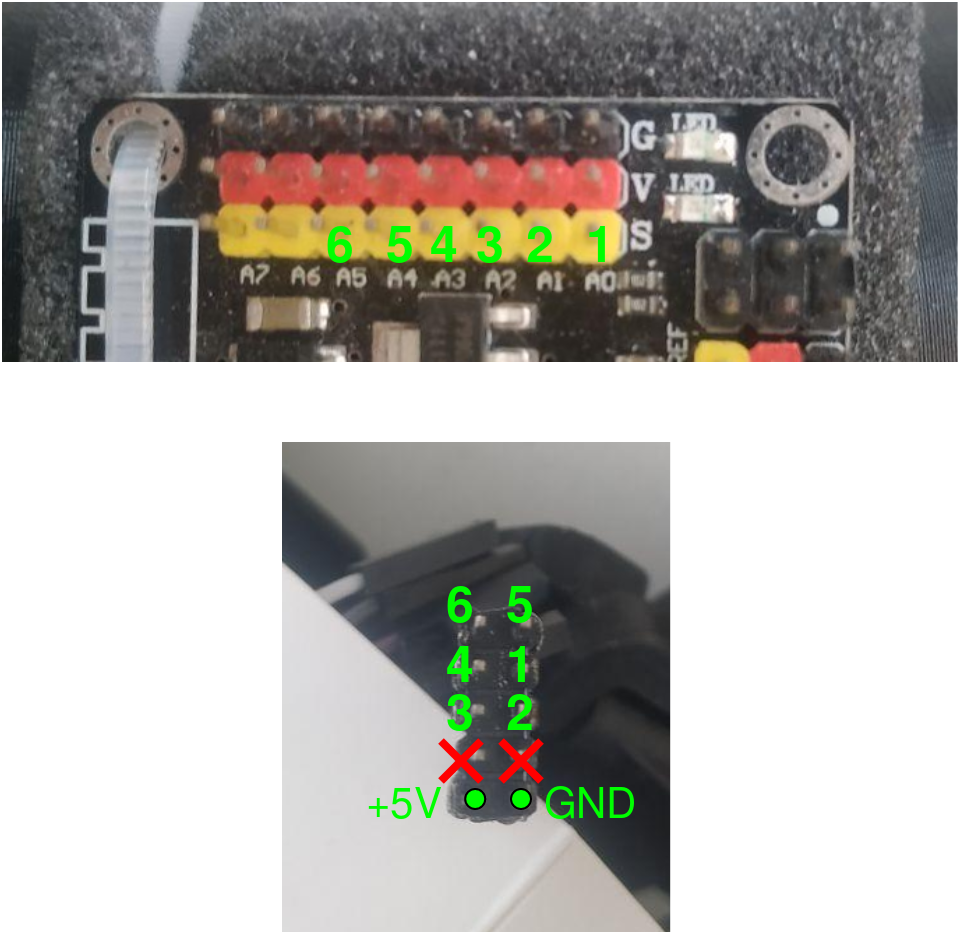
\includegraphics[scale=0.28]{./image/inst0.png}
\caption{Výstupy servomotorů}
\label{fig:Instr1}
\end{figure} 
 
\newpage
 
Připojte arduino v robotické ruce k externí desce (Obrázek \ref{fig:Instr2}).

 \begin{figure}[H]
\centering
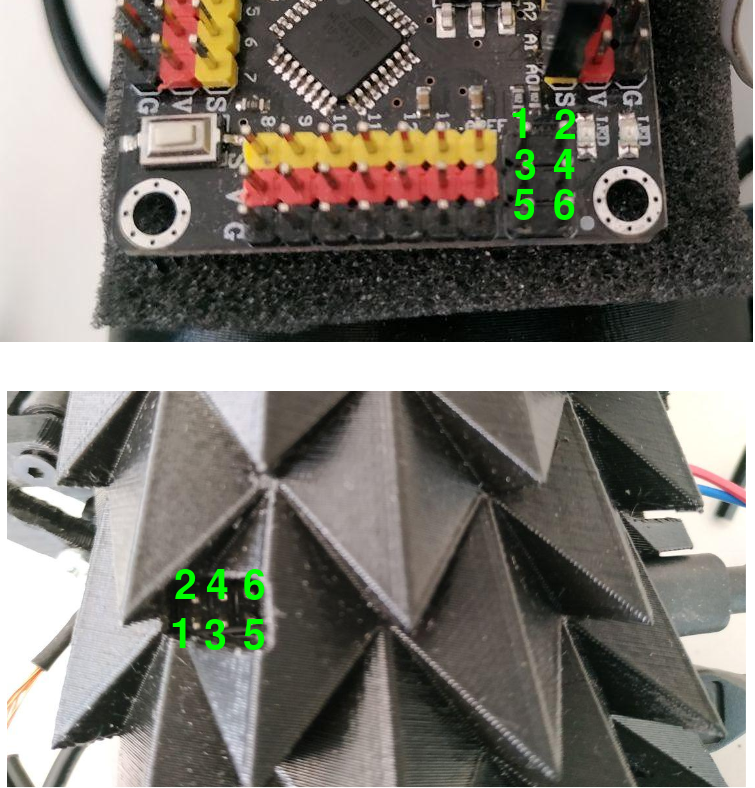
\includegraphics[scale=0.35]{./image/inst1.png}
\caption{Připojení desek}
\label{fig:Instr2}
\end{figure} 

\newpage

Připojte robotickou ruku k počítači a ke zdroji energie (powerbanka)\ref{fig:Instr3}.

 \begin{figure}[H]
\centering
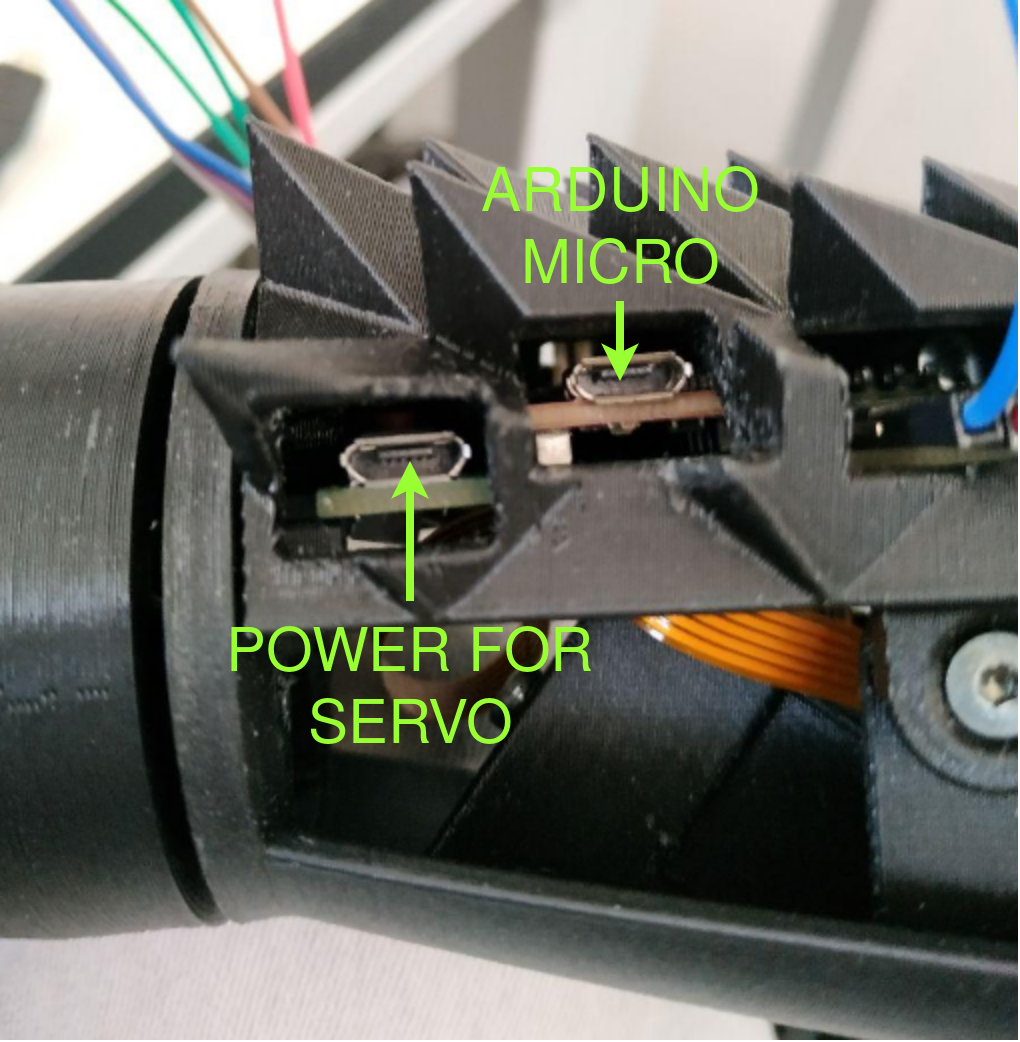
\includegraphics[scale=0.25]{./image/inst2.png}
\caption{Připojení robotické ruky}
\label{fig:Instr3}
\end{figure} 
\section{Funkce knihovny}


Knihovna je napsána v jazyce C a má následující funkce:

\hspace{2cm}

\texttt{init\_serial(SSerial *term)}


Funkce provede nastavení pro komunikaci se zařízením a uloží původní nastavení. Parametr \texttt{term} je struktura pro uložení nastavení.


\hspace{2cm}


\texttt{destr\_serial (SSerial *term)}


Funkce vrací původní nastavení.


\hspace{2cm}

\texttt{set\_io\_speed (int tty\_fd, SSerial *term)}


Funkce nastavuje výstupní/vstupní přenosovou rychlost a piny RTS a DTR sériového portu. Parametr \texttt{tty\_fd} určuje adresu zařízení. Parametr \texttt{term} určuje nastavení komunikace.

\hspace{2cm}

\texttt{open\_device (SArdDev* dev, const char* addr)}


Funkce inicializuje zařízení na adrese \texttt{addr} do struktury \texttt{dev}.

\hspace{2cm}


\texttt{close\_device (int tty\_fd, SSerial *term)}

Funkce ukončí komunikaci se zařízením.

\hspace{2cm}

\texttt{read\_from\_device (SArdDev dev, char* buff, int size)}

Funkce přečte data odeslaná zařízením \texttt{dev} a uloží je do \texttt{buff}. Parametr \texttt{size} určuje velikost buffru pro čtení.

\hspace{2cm}

\texttt{read\_glove\_position (SArdDev dev, char* buff, int size, bool wait\_glove)}

Funkce přečte aktuální polohu prstu připojené rukavice. 

\hspace{2cm}

\texttt{write\_to\_device (SArdDev* dev, char* buff, int size)}

Funkce odeslila data z  \texttt{buff} do zařízení \texttt{dev}.

\hspace{2cm}


\texttt{send\_states\_to\_hand (SArdDev* dev, int states[6])}

Funkce posílá pozice servomotorů do robotcké ruky z pole \texttt{states}. 


\hspace{2cm}


\texttt{resend\_data\_between\_device (SArdDev* from\_device, SArdDev* to\_device)}

Funkce přeposílá data ze zařízení \texttt{from\_device} do zařízení \texttt{to\_device}.

\hspace{2cm}

\texttt{open\_hand (SArdDev* dev)}

Funkce otevře robotickou ruku.

\hspace{2cm}

\texttt{close\_hand (SArdDev* dev)}

Funkce zavře robotickou ruku.

\chapter{Fotografie z testování}

Následující podkapitoly obsahují fotografie z testování modelu.

\section{Testování možností modelu}

Fotografie ke Kapitole \ref{ch:test}.

 \begin{figure}[H]
\centering
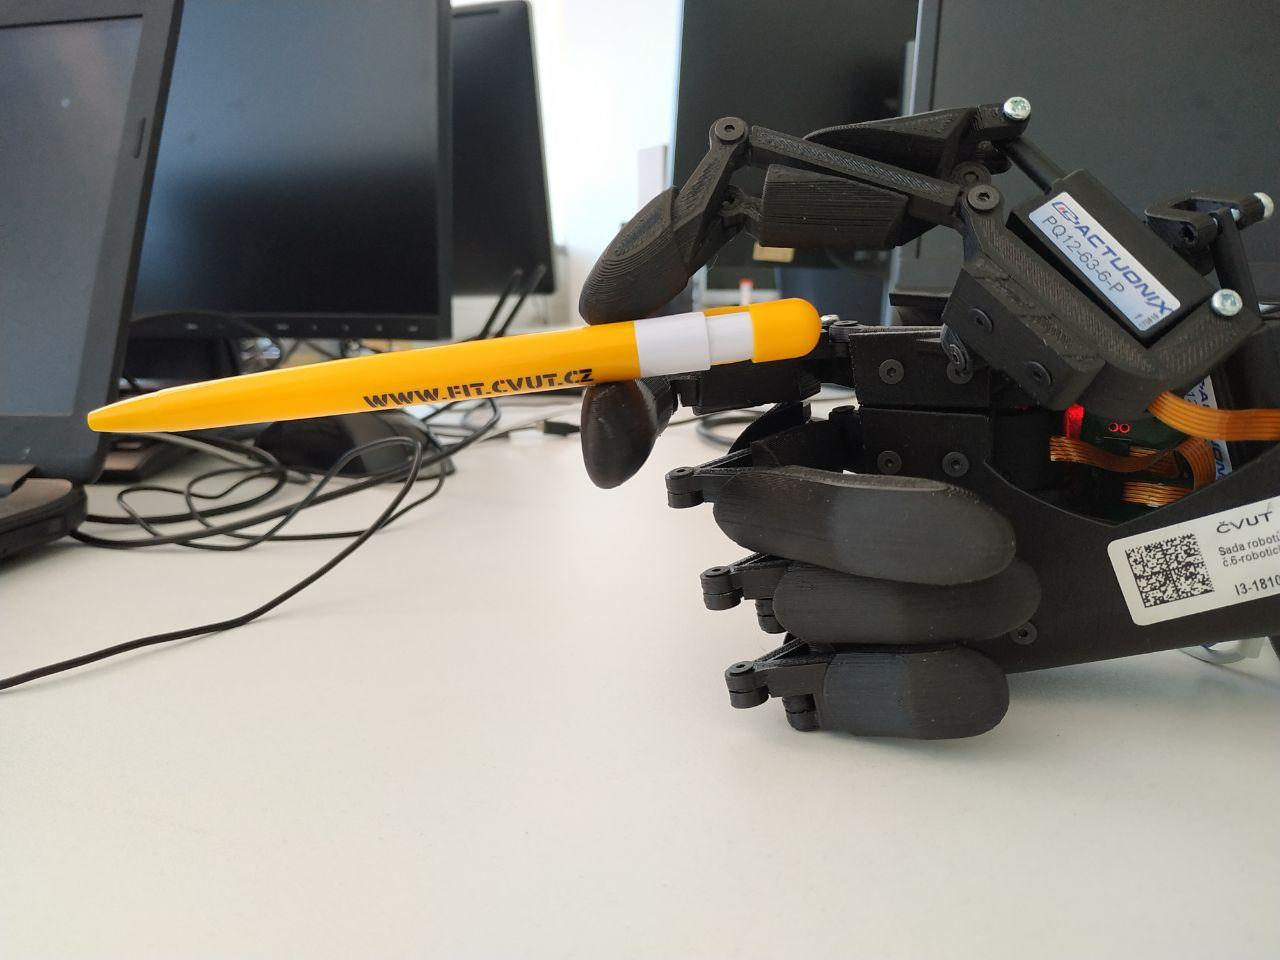
\includegraphics[scale=0.3]{./image/testF1.jpg}
\end{figure} 


 \begin{figure}[H]
\centering
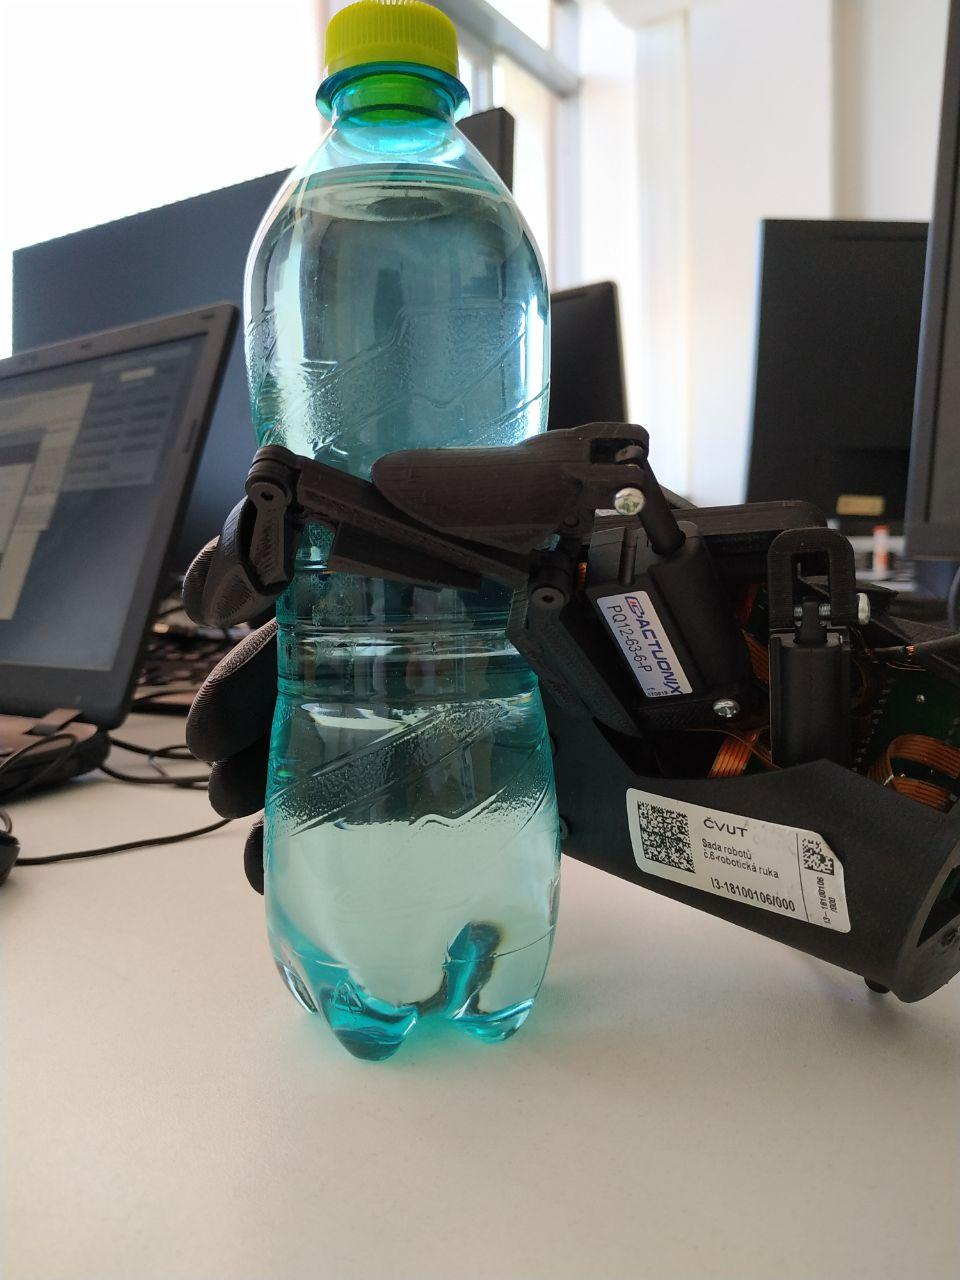
\includegraphics[scale=0.3]{./image/testF2.jpg}
\end{figure} 

 \begin{figure}[H]
\centering
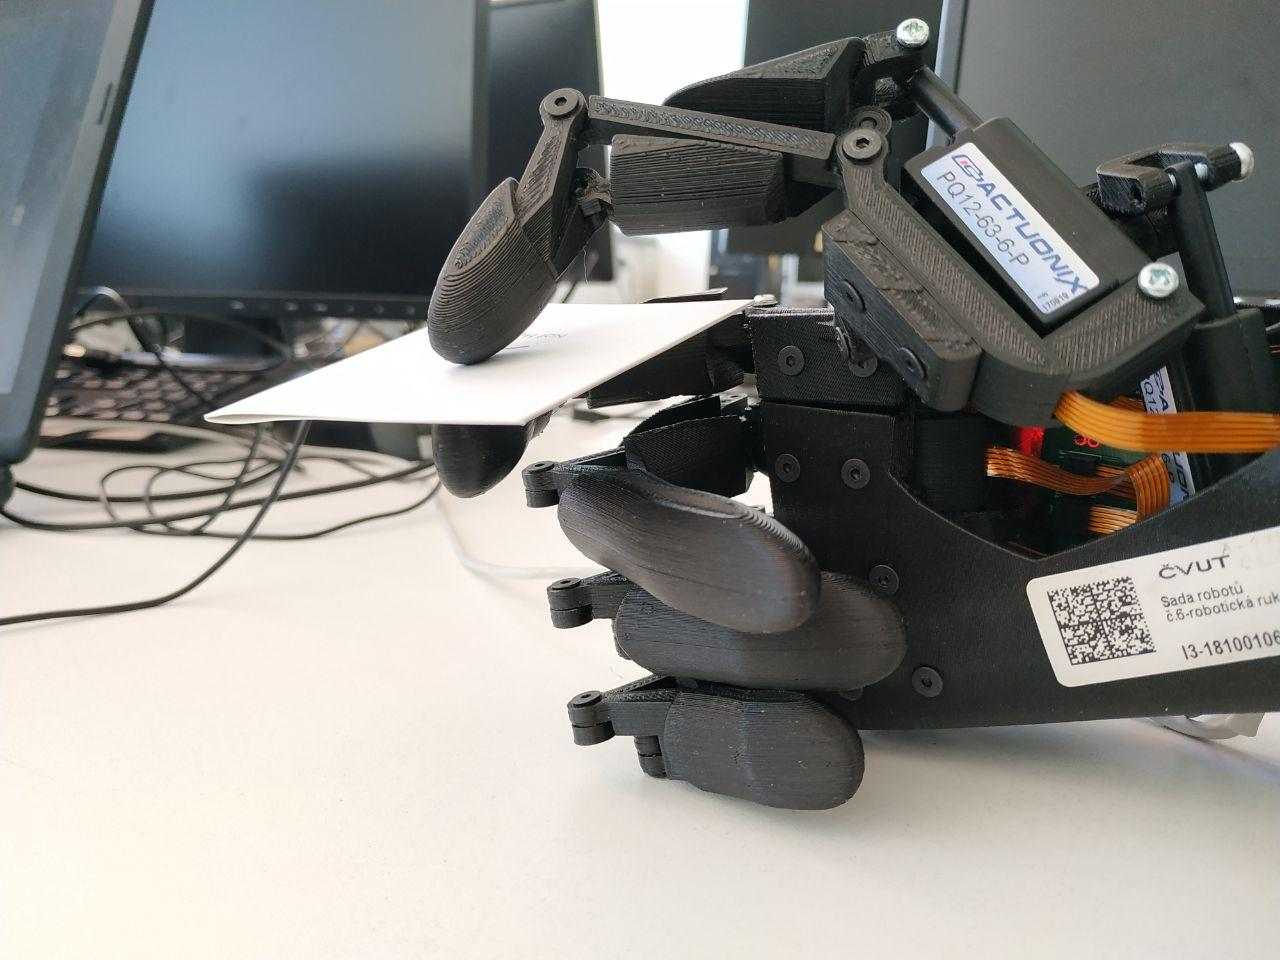
\includegraphics[scale=0.3]{./image/testF3.jpg}
\end{figure} 

 \begin{figure}[H]
\centering
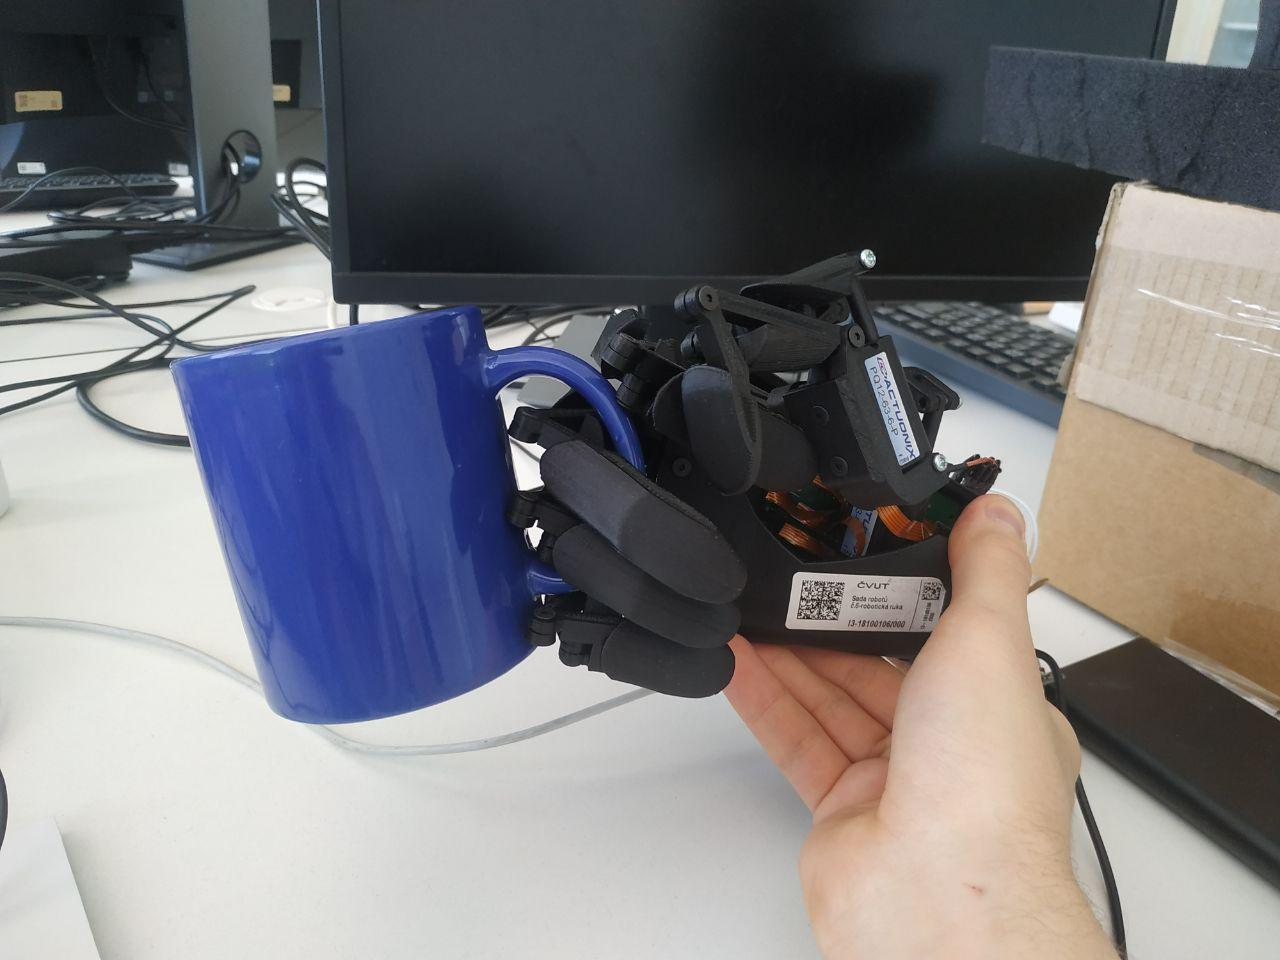
\includegraphics[scale=0.3]{./image/testF4.jpg}
\end{figure} 

\section{Testování řešení}

Fotografie ke Kapitole \ref{ch:testSol}.



 \begin{figure}[H]
\centering
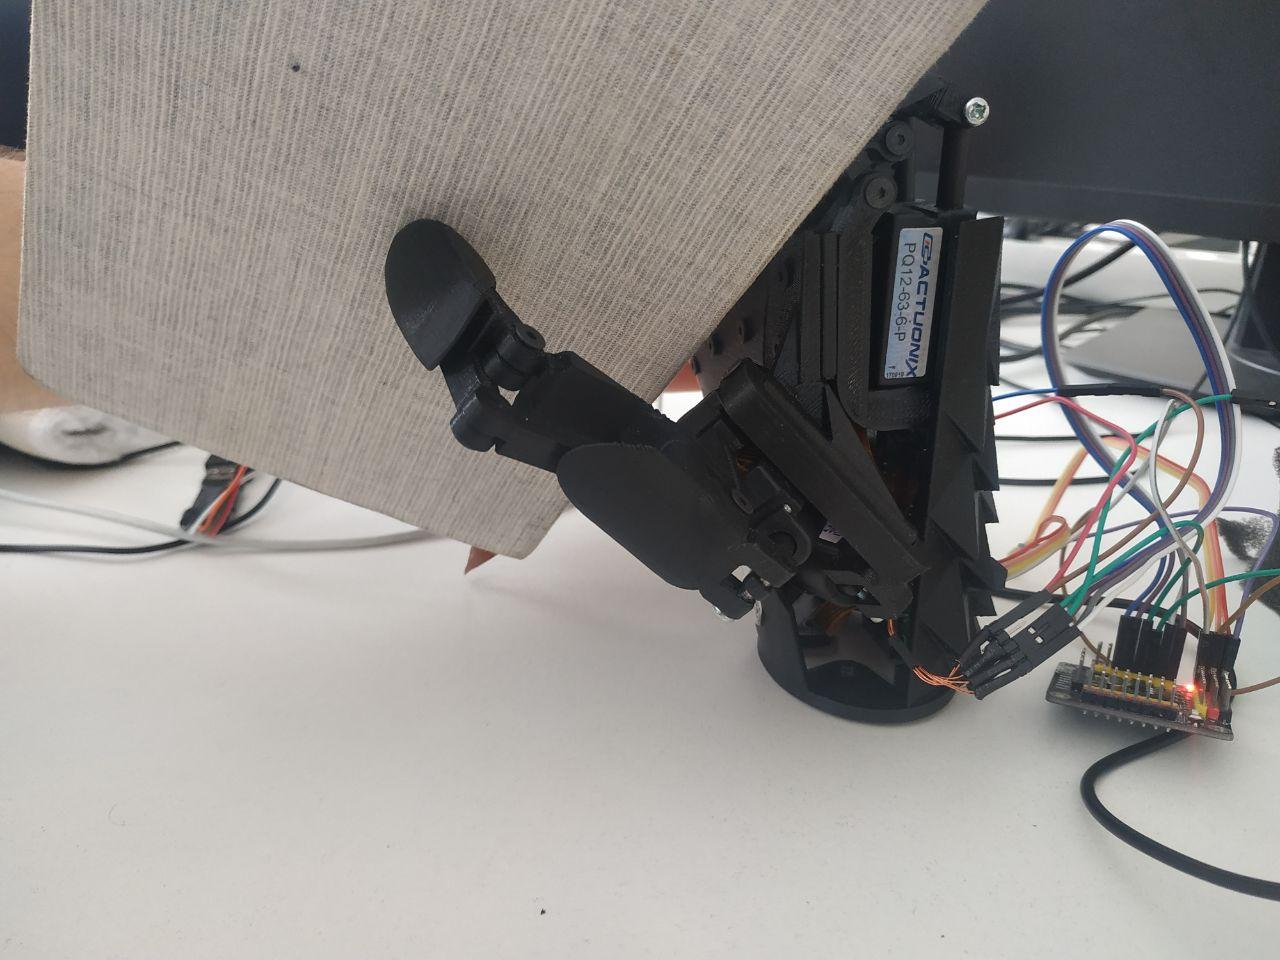
\includegraphics[scale=0.3]{./image/testSolF1.jpg}
\end{figure} 



 \begin{figure}[H]
\centering
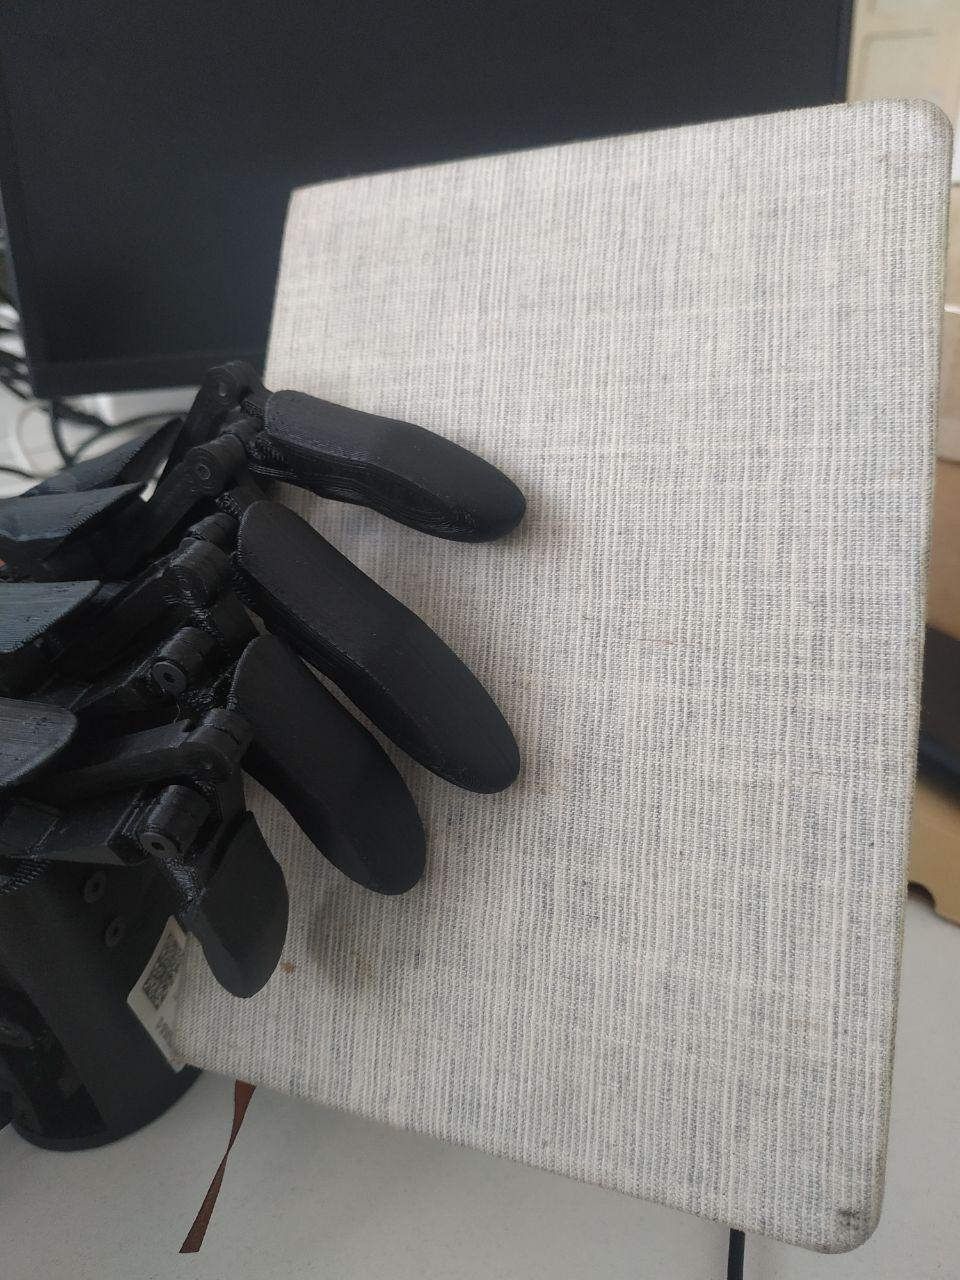
\includegraphics[scale=0.3]{./image/testSolF2.jpg}
\end{figure} 


 \begin{figure}[H]
\centering
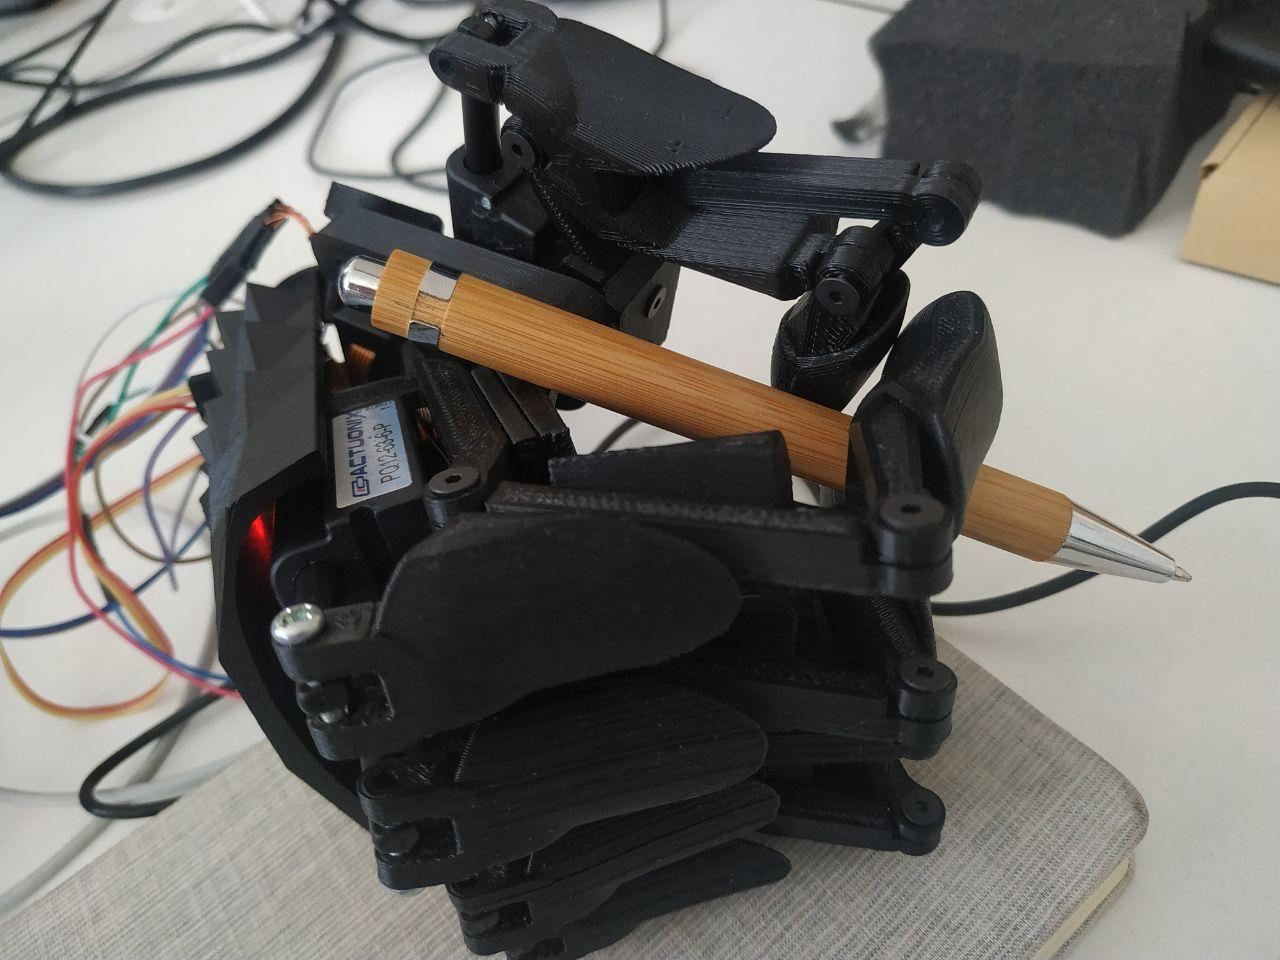
\includegraphics[scale=0.3]{./image/testSolF3.jpg}
\end{figure} 



 \begin{figure}[H]
\centering
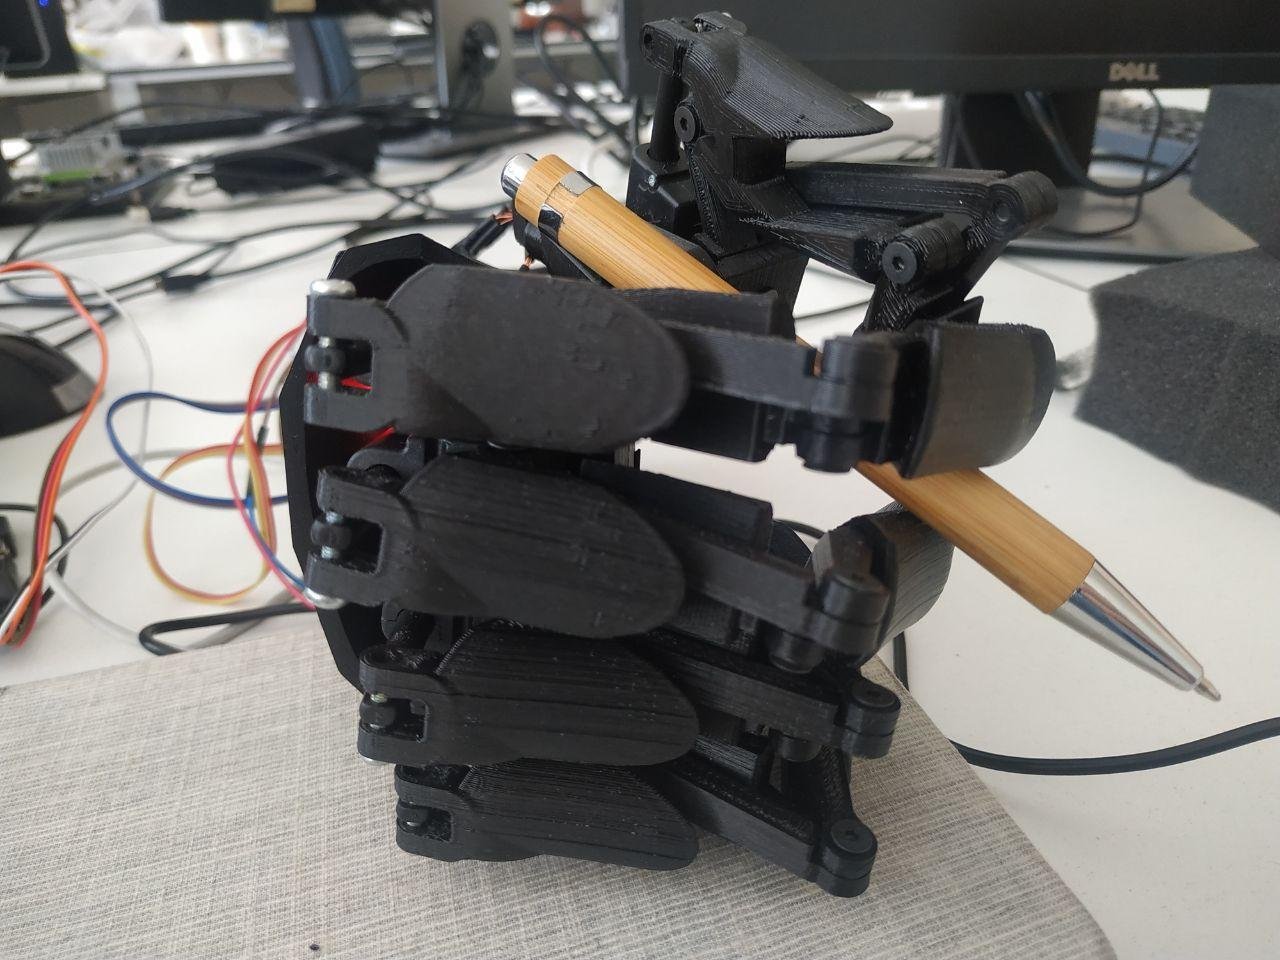
\includegraphics[scale=0.3]{./image/testSolF4.jpg}
\end{figure} 



 \begin{figure}[H]
\centering
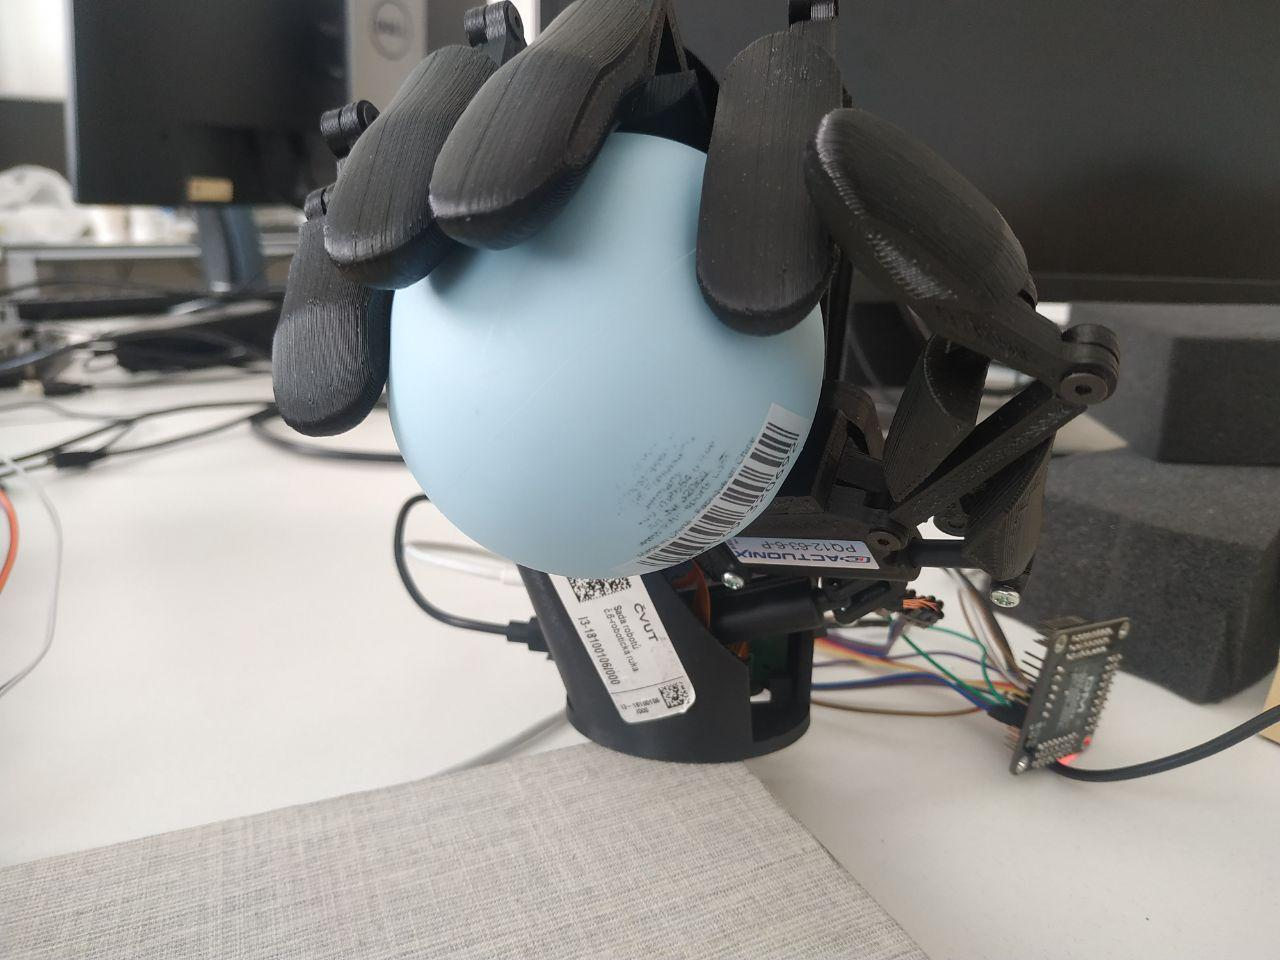
\includegraphics[scale=0.3]{./image/testSolF5.jpg}
\end{figure} 



\chapter{Seznam použitých zkratek}
% \printglossaries
\begin{description}
	\item[USB] Universal Serial Bus
	\item[LED] Light-emitting diode
	\item[IDE] Integrated Development Environment
	\item[PWM] Pulzně šířková modulace
	\item[ICSP] In-Circuit Serial Programming
	\item[SPI] Serial Peripheral Interface
	\item[MISO] Master In Slave Out
	\item[MOSI] Master Out Slave In	
	\item[SCLK] Serial Clock
	\item[SS] Slave Select
	\item[UART] Universal asynchronous receiver-transmitter	
	\item[USART] Universal synchronous and asynchronous receiver-transmitter	
	\item[XML] Extensible Markup Language
	\item[GUI] Graphical user interface
\end{description}


\chapter{Obsah přiloženého CD}

%upravte podle skutecnosti

\begin{figure}
	\dirtree{%
		.1 readme.txt\DTcomment{stručný popis obsahu CD}.
		.1 src.
		.2 impl\DTcomment{zdrojové kody implementace}.
		.2 documentation \DTcomment{dokumentace ke zdrojovým kódu aplikace}.
		.2 BP\_Popov\_Ilia\_2020\DTcomment{zdrojová forma práce ve formátu \LaTeX{}}.
		.1 text\DTcomment{text práce}.
		.2 BP\_Popov\_Ilia\_2020.pdf\DTcomment{text práce ve formátu PDF}.
		.1 videos\DTcomment{videa testování projektu}.
		.1 schemes\DTcomment{implementovaná schémata připojení}.
	}
\end{figure}




\end{document}
